\documentclass[12pt,openany,oneside]{book}
\usepackage[notlof,notlot,nottoc]{tocbibind}
\usepackage{graphicx}
\usepackage{hyphenat}
\usepackage{natbib}
%\usepackage{cite}
\usepackage{url}
\pagestyle{headings}
\setcounter{secnumdepth}{3}
\setcounter{tocdepth}{3}
\renewcommand{\contentsname}{Table of Contents}
\newcommand{\ticite}[1]{\textit{#1}}
\newcommand{\tiw}[1]{\mbox{#1}}
\newcommand{\ticode}[1]{\texttt{#1}}
\newcommand{\ticommand}[1]{\texttt{#1}}
\newcommand{\tisamp}[1]{`\texttt{#1}'}
\newcommand{\tikbd}[1]{\textsl{\texttt{#1}}}
%\newcommand{\tiref}[1]{Section~\ref{#1} [#1], page~\pageref{#1}}
\newcommand{\tiref}[1]{#1, page~\pageref{#1}}
\newcommand{\tixref}[1]{see Section~\ref{#1}: #1, page~\pageref{#1}}
\newcommand{\tipxref}[1]{see [#1], page~\pageref{#1}}
\newdimen{\standardmargin}  \setlength{\standardmargin}{15pt}
\newenvironment{display}[1][\standardmargin]%
                       {\begingroup\def~{\mbox{ }}\let\\=\lb
                        \list{}{\listparindent0pt  \itemindent0pt
                        \rightmargin0pt    \leftmargin#1}%
                \item}
               {\endlist\endgroup}

\newenvironment{tiexample}{\begin{display}\ttfamily\obeylines\vskip\parskip\parskip=0pt}{\end{display}}

\newsavebox{\savepar}
\newenvironment{ticartouche}{\begin{lrbox}{\savepar}
\begin{minipage}{.98\hsize}}
{\end{minipage}\end{lrbox}\noindent\fbox{\usebox{\savepar}}}

\usepackage[margin=1in]{geometry}
\usepackage{textcomp}
\newcommand{\registeredsymbol}{\textsuperscript{\textregistered}}
\usepackage{parskip}
%\usepackage{fancybox}
\usepackage{fancyvrb}
\usepackage{longtable}
\usepackage{needspace}
\usepackage[bookmarks=true,colorlinks=true,linktoc=page,linkcolor=blue,citecolor=blue]{hyperref}
\begin{document}

%\title{USF Neural Simulator}
%\author{Russell O'Connor}
%\maketitle
\pagenumbering{alph}

\begin{titlepage}
\begingroup
\parindent=0pt
\vglue1.85in
\font\titlefont=cmbx12 scaled \magstep 3
\leftline{\titlefont USF Neural Simulator}
\vskip4pt \hrule height 4pt width \hsize \vskip4pt
\vskip4pt \hrule height 2pt width \hsize \vskip2pc
\par\vfill
\pagebreak
\thispagestyle{empty}
\vglue 0pt plus 1filll
Copyright (C) 2003,2007,2011 Bruce G. Lindsey
\endgroup
\end{titlepage}
\pagenumbering{roman}

\tableofcontents

\chapter{Overview}
\pagenumbering{arabic}

The USF Neural Simulator\footnote{The program was developed in laboratory of
B. G. Lindsey at the University of South Florida by U.J. Balis,
Kendall Morris and others using Fortran, the K\&R C language, X-windows
and Motif. The latest version was modified and enhanced as described
in this document by Russell O'Connor in 2005-2007. Development of the
program was supported by NIH grants NS19814 and NS46062 as part of the
NSF/NIH Collaborative Research in Computational Neuroscience Program.}
started out as an implementation of Ronald J.  MacGregor's SYSTM11
simulator as documented in his 1987 book \ticite{Neural and Brain
Modeling}, together with the NEWSNED network editor and the SNEDSKOP
waveform display program.  It has now been rewritten in the C
language.  The new program is compatible with the previous program's
functionality, and has many new features.

The software is written for the UNIX environment.  The UNIX
environments it has been run on include Linux, Cygwin on Windows, and
HP-UX.

The input to the simulator is in two forms: the first is a ``.sim''
format text file that lists the values of all the parameters, and the
second is answers to questions that the simulator asks on the command
line.  The answers can be listed in advance in a second text file and
then fed to the simulator.  These files could be created by hand in
any text editor (run Cygwin's dos2unix on them if you use a Windows
program to create them), but NEWSNED provides a graphical interface
for drawing the network, specifying the parameters, creating the two
files, and invoking the simulator, that makes the process much easier.

The output from the simulator is in the form of a ``.bdt'' format text
file that lists the spike times of selected cells and the integrated
activity of a population, and ``wave'' text files that record selected
membrane potentials and other values for display by SNEDSKOP.  The
``.bdt'' files can be displayed with the ``scope'' application, also
available from this laboratory.

\chapter{Installation}


\section{Installing on Windows}


\subsection{The Cygwin UNIX Environment}

In order to run the simulator on Windows, you first need to install
the Cygwin UNIX environment, which is available at no cost from
\url{http://www.cygwin.com}.  Installation instructions are available
at that website, and a few additional details are in the next section
of this manual.





\subsection{Installing Cygwin}

The Cygwin environment is installed using the Cygwin installer
program, \ticode{setup.exe}, which can be downloaded from
\url{http://www.cygwin.com/setup.exe}.  Run the program, and you will
be presented with a series of dialog boxes asking questions, as is
typical for Windows software install programs.  The default responses
for most of the questions are correct for most installations, but you
will need to make a choice at the ``Choose Download Site'' screen
and the ``Select Packages'' screen.

The Cygwin software is available from nearly 100 download sites
worldwide but many of the sites are slow or unavailable at any
particular time.  Choosing a site from the list is mostly a matter of
trying one and seeing how it works.  The site
\url{http://cygwin.paracoda.com/} has been fast and reliable here
lately (October 11, 2005 in Tampa, FL).

By default, Cygwin setup installs a minimal set of packages.  In order
to run the simulator, you will need more than that.  The easiest thing
to do it to install all the packages, if you have the disk space.  The
total disk space requirement is, as of October 11, 2005, 2.4 gigabytes
plus 1.25 gigabytes for the package files (which can be deleted after
installation).  The procedure for installing all the packages is
documented at \url{http://www.cygwin.com/faq/faq.setup.html}.  The key
paragraph is:

\begin{quote}
At the ``Select Packages'' screen, in ``Categories'' view, at the line
marked ``All'', click on the word ``default'' so that it changes to
``install''. (Be patient, there is some computing to do at this
step. It may take a second or two to register the change.) This tells
Setup to install everything, not just what it thinks you should have
by default.
\end{quote}

If you are short on disk space, you can install the default packages
plus at least the gcc, lesstif, xorg-x11-base, and xterm packages, but
I have not tried it so I don't know what other packages you may need,
or how much disk space you save.

After setup is finished, copy the file
\verb-C:\cygwin\usr\X11R6\bin\startxwin.bat- to your desktop so that
you can get at it easily.  Then double-click on it and you should get
a command-line window.  (If you installed Cygwin somewhere other than
\verb-C:\cygwin-, you will have to modify the above instruction
accordingly.)

\subsection{Installing the Simulator}

From this point on, installing the simulator on Windows is the same as
installing it on UNIX.  \tixref{UNIX Install}.

\section{Installing on UNIX}\label{UNIX Install}

In order to install the simulator on UNIX, your UNIX system must have
a C compiler, the X Window System and the Motif (of Lesstif) GUI
libraries.

The simulator is packaged in a .tar.gz file.  Copy this file (for
example, the file named \tisamp{simulator-0.1.28.tar.gz}) to the directory under which
you would like to install the simulator.  For example, if you received
the file via email, you might save the attachment to
\verb-C:\cygwin\home\myname-. Then, at the cygwin command line,
\tikbd{cd} to that directory, and type something like the following:

\begin{tiexample}\tikbd{gunzip -c simulator-0.1.28.tar.gz | tar xf -}
\tikbd{cd simulator-0.1.28}
\tikbd{./configure > configure.out}
\tikbd{make > make.out}
\tikbd{make install > make\_install.out}
\end{tiexample}

\noindent
You may need to have admin privileges for "make install" to work.

If it succeeds, you can invoke NEWSNED by typing:

\begin{tiexample}
\ticommand{newsned}
\end{tiexample}

\chapter{Running the Simulator}


\section{Model Parameters}
\label{Parameters}

The model parameters can be specified either by using NEWSNED or by
editing the ``.sim'' file.  There are two formats of ``.sim'' file.
The simulator will read either format, but NEWSNED only writes the new
format.  The labels used for the parameters are different in NEWSNED
than they are in the ``.sim'' files.  In the following sections, each
parameter is described and the labels used in NEWSNED and in the
``.sim'' files, and the variable names used in \ticite{Neural and Brain
Modeling},
%iftex
and the symbols used in Breen et al,
%end iftex
are given in the following format:

\begin{flushleft}
\begin{tabular}{@{}ll@{}}
SNED:  &  label used in NEWSNED\\
SIM:  &  label used in the old format ``.sim'' file\\
SIM2:  &  label used in the new format ``.sim'' file\\
%iftex
BREEN: & label used in Breen et al (\tipxref{Breen et al})\\
%end iftex
VAR:  &  variable name used in {\ticite{Neural and Brain Modeling}}\\
UNIT:  &  unit of measure for the parameter\\
TYP:  &  typical values for the parameter\\
\end{tabular}
\end{flushleft}

If a particular entry does not appear for a particular parameter, that
parameter is not used in that place.

%iftex
%ignore
%end iftex

%The labels used in SIM2 are similar to the symbols used in Breen et
%al, so can be used to relate the simulator model parameters to the
%parameters in Breen et al.  Otherwise, the PDF version of this manual
%lists Breen's symbols as well.

%iftex
%end ignore
%end iftex

Several of the parameter descriptions refer to variables that decay
exponentially toward a value, with a specified time constant.  That
means that the variable is governed by an equation of the form

\begin{tiexample}
$A + (V - A) * exp (-t / t0)$
\end{tiexample}

\noindent
where t0 is the time constant and A is the value toward which the
variable is decaying.  (V is the value of the variable at t = 0).


%iftex
\vspace{\fill}
%end iftex

%need 2000
\subsection{MacGregor Cell Parameters}
\label{MacGregor Parameters}

\begin{flushleft}
\begin{tabular}{@{}ll@{}}
SNED:  &  Accommodation Time\\
SIM:  &  Time constant for accommodation\\
SIM2:  &  DCTH\\
VAR:  &  TTH\\
UNIT:  &  milliseconds\\
TYP:  &  20-{}25\\
\end{tabular}
\end{flushleft}

\noindent
The firing threshold moves up and down in proportion to membrane
potential changes, but it doesn't move immediately to the new value.
Instead, it approaches it exponentially.  This parameter is the time
constant of the exponential decay toward the new value, except for
SIM2, where it is exp(-step / TTH).
\filbreak
\vspace{\baselineskip}

%need 2000
\label{TGK}
\begin{flushleft}
\begin{tabular}{@{}ll@{}}
SNED:  &  Potassium Conductance Time\\
SIM:  &  Time constant for potassium conductance\\
SIM2:  &  TGK\\
VAR:  &  TGK\\
UNIT:  &  milliseconds\\
TYP:  &  3-10\\
\end{tabular}
\end{flushleft}

\noindent
In the absence of spikes, the potassium conductance decays
exponentially toward zero with the time constant specified by this
parameter.  This controls the refractory period.  During a spike, the
potassium conductance decays exponentially toward a specified value
(\tipxref{B}), with this same time constant.  If this parameter is set
to 0, the cell model changes to Hybrid IF (\tipxref{Hybrid IF Parameters}).
\filbreak
\vspace{\baselineskip}

\label{TMEM}
%need 2000
\begin{flushleft}
\begin{tabular}{@{}ll@{}}
SNED: & Membrane Time Constant\\
SIM: & Time constant for membrane potential\\
SIM2: & TMEM\\
VAR: & TMEM\\
UNIT: & milliseconds\\
TYP: & 5-11\\
\end{tabular}
\end{flushleft}
\noindent
In the absence of potassium or synaptic conductances, the membrane
potential will decay exponentially toward its resting potential (which
is taken as 0 in this model) with the time constant specified by this
parameter.  If this parameter is set to 0, the cell model changes to a
PSR model (\tipxref{PSR Parameters}).
\filbreak
\vspace{\baselineskip}

%need 2000
\begin{flushleft}
\begin{tabular}{@{}ll@{}}
SNED: & Resting Threshold\\
SIM: & Resting threshold\\
SIM2: & Th0\\
VAR: & THO\\
UNIT: & millivolts\\
TYP: & 10-20\\
\end{tabular}
\end{flushleft}
\noindent
When the membrane potential has been at its resting value so that the
firing threshold is not affected by accommodation, the firing
threshold will have the value specified by this parameter, relative to
the resting membrane potential.  If the value of this parameter in
NEWSNED's Cell Population Definition Panel is followed by a slash and
a second number, the value of this parameter will be distributed
around the specified value (the first number) with a normal
distribution with a standard deviation equal to the second number.
\filbreak
\vspace{\baselineskip}

%need 2000
\label{B}
\begin{flushleft}
\begin{tabular}{@{}ll@{}}
SNED: & K conductance change with AP\\
SIM: & Change in potassium conductance with action potential\\
SIM2: & B\\
VAR: & B\\
UNIT: & dimensionless\\
TYP: & 25-27\\
\end{tabular}
\end{flushleft}
\noindent
During an action potential (which has a duration of one time step),
the potassium conductance will decay exponentially toward this value.
This value is in units of the resting membrane conductance.  In other
words, a value of 2 means twice the resting membrane conductance.
\filbreak
\vspace{\baselineskip}

%need 2000
\begin{flushleft}
\begin{tabular}{@{}ll@{}}
SNED: & Accommodation Parameter\\
SIM: & Accommodation parameter\\
SIM2: & MGC\\
VAR: & C\\
UNIT: & dimensionless\\
TYP: & .04-.85\\
\end{tabular}
\end{flushleft}
\noindent
As the membrane potential rises above its resting value (taken to be 0
in this model), the firing threshold will eventually rise in
proportion from its resting value.  This parameter is the
proportionality constant.  For example, if this parameter is .5, then
when the membrane potential rises 2 mV above its resting potential,
the firing threshold will rise exponentially toward 1 mV above its
resting value, with a specified time constant (see TTH, above).
\filbreak
\vspace{\baselineskip}

%need 2000
\begin{flushleft}
\begin{tabular}{@{}ll@{}}
SNED: & Population Size\\
SIM: & Number of cells in population\\
SIM2: & cell\_count\\
VAR: & N\\
UNIT: & count\\
TYP: & 1-1000\\
\end{tabular}
\end{flushleft}
\noindent
All the cells in a population have the same values of the other parameters
specified in this section, but each cell in the population can have a
different membrane potential and firing pattern because it can
have a different firing pattern at its synapses than the other cells
in the population, so each cell is simulated separately.  This
parameter specifies how may cells in the population are simulated.
\filbreak
\vspace{\baselineskip}

\begin{flushleft}
\begin{tabular}{@{}ll@{}}
SNED: & DC Injected Current\\
SIM: & dc injected current for each population\\
SIM2: & GE0\\
VAR: & SC\\
UNIT: & millivolts\\
TYP: & 0-17\\
\end{tabular}
\end{flushleft}
\noindent
An injected current will raise the membrane potential by an amount
that is inversely proportional to the membrane conductance.  Instead
of being specified directly as a current, the ``DC Injected Current''
is specified in terms of the effect it has on the membrane potential.
This parameter is specified in millivolts, and it is interpreted as
the current that is required to raise the membrane potential by the
specified number of millivolts when the membrane conductance has its
resting value.  The effect on the membrane potential at other membrane
conductances will be inversely proportional to the conductance.
\filbreak
\vspace{\baselineskip}

%need 2000
\begin{flushleft}
\begin{tabular}{@{}ll@{}}
SNED: & Cell Population Comment\\
SIM: & [unused]\\
SIM2: & [unused]\\
VAR: & [unused]\\
UNIT: & n/a\\
TYP: & n/a\\
\end{tabular}
\end{flushleft}
\noindent
This is not really a simulation parameter, but instead is just a label for a cell
population on NEWSNED's graphical display.  It does not appear in the
``.sim'' file.  It is listed here because it appears in NEWSNED on the
cell population parameters screen.
\filbreak
\vspace{\baselineskip}

%need 2000
\begin{flushleft}
\begin{tabular}{@{}ll@{}}
SNED: & [implicit]\\
SIM: & Number of targets of cell populations\\
SIM2: & targetpop\_count\\
VAR: & NTGR\\
UNIT: & count\\
TYP: & n/a\\
\end{tabular}
\end{flushleft}
\noindent
This parameter is the number of connections between populations whose
source is this cell population.  This is not explicitly entered in
NEWSNED, because NEWSNED determines it from the network drawing.  A
single ``connection between populations'' represents a connection from
each cell of the source population to some number of cells of the
target population.  There can be multiple ``connections between
populations'' from the same source population to the same target
population, and each of those connections is counted separately for
this parameter.  However, if you set up multiple connections that all
have the same source and target population, NEWSNED will only allow
you to edit the parameters of the first of the connections.
\filbreak
\vspace{\baselineskip}

%need 2000
\begin{flushleft}
\begin{tabular}{@{}ll@{}}
SNED: & Noise Amplitude\\
SIM2: & noise\_amp\\
UNIT: & nanosiemens\\
TYP: & 0 - .3\\
\end{tabular}
\end{flushleft}
\noindent
Each cell has an internal noise generator that acts like two synapses,
one with an equilibrium potential of 70 mV above resting and the other
with -70mV.  Each acts like it has an incoming firing probability of
.05 per time step, and a synapse time constant of 1.5ms.  This
parameter is the conductance that gets added to the synapse
conductance on each (virtual) spike.
\filbreak
\vspace{\baselineskip}

\subsubsection*{Unused Parameters}

The old format ``.sim'' file specifies several cell population
parameters that are not used in this version of the simulator.  Their
values in the ``.sim'' file have no effect on the simulation.  The
labels for these parameters as they appear in the sim file are as
follows:

\begin{tiexample}
\begin{samepage}Rebound parameter:
Rebound time constant:
Threshold for removal of ika inactivation:
Threshold for ika activation:
Maximum ika conductance:
Proportionality constant for removal of ika inactivation:
Proportionality constant for ika activation:
Time constant for ika:
\end{samepage}
\end{tiexample}

\subsection{Hybrid IF Cell Parameters}
\label{Hybrid IF Parameters}

If the Potassium Conductance Time of the MacGregor model (\tipxref{TGK})
is set to 0, the cell model changes to Hybrid IF (``burster'').  The
Hybrid IF model is derived from the model described in
\begin{quote}
\label{Breen et al} Barbara J. Breen, William C. Gerken, Robert
J. Butera, Jr., Hybrid integrate-and-fire model of a bursting neuron,
\ticite{Neural Computation, v.15} n.12, p.2843-2862, December 2003.
\end{quote}

\noindent The TYP values shown below are from Breen et al.  If we have
used a different value, it is shown in parentheses.

There is no description of these parameters unless the description
differs from the parameter used in Breen et al.

If a parameter that appears on the NEWSNED Cell Population Definition
Panel for a Hybrid IF population does not appear in this list, it is
documented under the MacGregor Parameters (\tipxref{MacGregor Parameters}).

%need 2000
\begin{flushleft}
\begin{tabular}{@{}ll@{}}
SNED: & Time Constant for h\\
SIM2: & taubar\_h\\
%iftex
BREEN: & $\bar\tau_h$\\
%end iftex
UNIT: & milliseconds\\
TYP: & 10,000 (2,000)\\
\end{tabular}
\end{flushleft}
\filbreak
\vspace{\baselineskip}

%need 2000
\begin{flushleft}
\begin{tabular}{@{}ll@{}}
SNED: & NaP conductance\\
SIM2: & g\_NaP\_h\\
%iftex
BREEN: & $g_{\rm NaP-h}$\\
%end iftex
UNIT: & nanosiemens\\
TYP: & 2.8 (3)\\
\end{tabular}
\end{flushleft}
\filbreak
\vspace{\baselineskip}

%need 2000
\begin{flushleft}
\begin{tabular}{@{}ll@{}}
SNED: & Half-voltage for h\\
SIM2: & theta\_h\\
%iftex
BREEN: & $\Theta_h$\\
%end iftex
UNIT: & millivolts\\
TYP: & -48 (-51)\\
\end{tabular}
\end{flushleft}
\filbreak
\vspace{\baselineskip}

%need 2000
\begin{flushleft}
\begin{tabular}{@{}ll@{}}
SNED: & Slope for h\\
SIM2: & sigma\_h\\
%iftex
BREEN: & $\sigma_h$\\
%end iftex
UNIT: & millivolts\\
TYP: & 6 (5)\\
\end{tabular}
\end{flushleft}
\filbreak
\vspace{\baselineskip}

%need 2000
\begin{flushleft}
\begin{tabular}{@{}ll@{}}
SNED: & Half-voltage for activation\\
SIM2: & theta\_m\\
%iftex
BREEN: & $\Theta_{m-\rm NaPh}$\\
%end iftex
UNIT: & millivolts\\
TYP: & -40 (-43)\\
\end{tabular}
\end{flushleft}
\filbreak
\vspace{\baselineskip}

%need 2000
\begin{flushleft}
\begin{tabular}{@{}ll@{}}
SNED: & Slope for activation\\
SIM2: & sigma\_m\\
%iftex
BREEN: & $\sigma_{m-\rm NaPh}$\\
%end iftex
UNIT: & millivolts\\
TYP: & -6\\
\end{tabular}
\end{flushleft}
\filbreak
\vspace{\baselineskip}

%need 2000
\begin{flushleft}
\begin{tabular}{@{}ll@{}}
SNED: & Reset Voltage @h=0\\
SIM2: & Vreset\\
%iftex
BREEN: & $V_{\rm Reset}(0)$\\
%end iftex
UNIT: & millivolts\\
TYP: & -47.359 (-42)\\
\end{tabular}
\end{flushleft}
\filbreak
\vspace{\baselineskip}

%need 2000
\begin{flushleft}
\begin{tabular}{@{}ll@{}}
SNED: & Threshold Voltage\\
SIM2: & Vthresh\\
%iftex
BREEN: & $V_{\rm Thresh}(h)$\\
%end iftex
UNIT: & millivolts\\
TYP: & (-37)\\
\end{tabular}
\end{flushleft}
\noindent In Breen et al, this parameter is a function of h.  In the simulator,
it is a constant.
\filbreak
\vspace{2\baselineskip}

%need 2000
\begin{flushleft}
\begin{tabular}{@{}ll@{}}
SNED: & Delta\_h @ h=0\\
SIM2: & delta\_h\\
%iftex
BREEN: & $\Delta h(0)$\\
%end iftex
UNIT: & dimensionless\\
TYP: & -0.00078 (0)\\
\end{tabular}
\end{flushleft}
\noindent
\filbreak
\vspace{\baselineskip}

%need 2000
\begin{flushleft}
\begin{tabular}{@{}ll@{}}
SNED: & Applied Current (Iapp)\\
SIM2: & GE0\\
%iftex
BREEN: & $I_{\rm app}$\\
UNIT: & picoamps\\
TYP: & 13-25 (0)\\
\end{tabular}
\end{flushleft}
\noindent
\filbreak
\vspace{\baselineskip}

%need 2000
\subsection{Pulmonary Stretch Receptor Parameters}
\label{PSR Parameters}

If the Membrane Time Constant of the MacGregor model (\tipxref{TMEM}) is
set to 0, the cell model changes to a PSR model.  The PSR model is
intended for modeling Pulmonary Stretch Receptors.  The steady-state
outgoing firing rate from a PSR cell is the same as the steady-state
incoming firing rate, but there is an exponential delay between
changes in the incoming firing rate and changes in the outgoing firing
rate.  Only the firing rate of the incoming connections matters, not
the strength or the equilibrium potential or the time constant.  The
firing rate is converted in the PSR model to a firing probability per
time step.

%need 2000
\begin{flushleft}
\begin{tabular}{@{}ll@{}}
SNED: & Rise Time\\
SIM2: & DCTH\\
UNIT: & milliseconds\\
TYP: & 500\\
\end{tabular}
\end{flushleft}
\noindent
If the incoming firing probability (IFP) is higher than the outgoing
firing probability (OFP), the outgoing firing probability is updated
on each time step as follows: $OFP = IFP + (OFP - IFP) * exp
(-step / RiseTime)$.  So the OFP will get most of the way up to the
IFP in ``Rise Time'' milliseconds.
\filbreak
\vspace{\baselineskip}

%need 2000
\begin{flushleft}
\begin{tabular}{@{}ll@{}}
SNED: & Fall Time\\
SIM2: & DCG\\
UNIT: & milliseconds\\
TYP: & 500\\
\end{tabular}
\end{flushleft}
\noindent
If the incoming firing probability (IFP) is lower than the outgoing
firing probability (OFP), the outgoing firing probability is updated
on each time step as follows: $OFP = IFP + (OFP - IFP) * exp
(-step / FallTime)$.  So the OFP will get most of the way down to the
IFP in ``Rise Time'' milliseconds.
\filbreak
\vspace{\baselineskip}

%need 2000
\begin{flushleft}
\begin{tabular}{@{}ll@{}}
SNED: & Output Threshold\\
SIM2: & Thr\\
UNIT: & dimensionless\\
TYP: & 0\\
\end{tabular}
\end{flushleft}
\noindent
The probability that there will be a spike on a particular time step
is calculated as $OFP - OutputThreshold$ (OFP = outgoing firing probability).
If the result is negative, there are no output spikes.
\filbreak
\vspace{\baselineskip}


%need 2000
\subsection{Fiber Population Parameters}
\label{Fiber Parameters}

%need 2000
\begin{flushleft}
\begin{tabular}{@{}ll@{}}
SNED: & Probability of Firing\\
SIM: & Probability of fiber population firing\\
SIM2: & probability\\
VAR: & P\\
UNIT: & dimensionless (probability)\\
TYP: & .01-.05\\
\end{tabular}
\end{flushleft}
\noindent
Each fiber in the population generates an action potential at each
time step with the probability specified by this parameter.
Therefore, if the time step in seconds is T, the average firing rate
of each fiber will be P/T.
\filbreak
\vspace{\baselineskip}

%need 2000
\begin{flushleft}
\begin{tabular}{@{}ll@{}}
SNED: & Time to begin firing\\
SIM: & Time fiber population begins firing\\
SIM2: & start\\
VAR: & INSTR\\
UNIT: & time steps\\
TYP: &\\
\end{tabular}
\end{flushleft}
\noindent
The probability of firing for all the fibers in the population is 0
until the time specified by this parameter, at which point the
``Probability of Firing'' parameter takes over.  This parameter is in
time steps from the start of the simulation.
\filbreak
\vspace{\baselineskip}

%need 2000
\begin{flushleft}
\begin{tabular}{@{}ll@{}}
SNED: & Time to end firing\\
SIM: & Time fiber population stops firing\\
SIM2: & stop\\
VAR: & INSTP\\
UNIT: & time steps\\
TYP: &\\
\end{tabular}
\end{flushleft}
The probability of firing for all the fibers in the population is 0
after the time specified by this parameter.  The ``Probability of
Firing'' parameter has no effect after this time.  This parameter is
in time steps from the start of the simulation.
\noindent
\filbreak
\vspace{\baselineskip}

%need 2000
\begin{flushleft}
\begin{tabular}{@{}ll@{}}
SNED: & Random Number Seed\\
SIM: & Random number seed for fiber population firing\\
SIM2: & infsed\\
VAR: & INFSED\\
UNIT: &\\
TYP: &\\
\end{tabular}
\end{flushleft}
\noindent
The firing patterns of the fibers in the population is determined by a
pseudo-random number generator, and this parameter determines the
sequence of numbers generated by the pseudo-random number generator.
The firing pattern will always be the same for the same value of this
parameter (but different for different fibers in the population).
Different fiber populations should have different values of this
parameter in order to generate different firing patterns.
\filbreak
\vspace{\baselineskip}

%need 2000
\begin{flushleft}
\begin{tabular}{@{}ll@{}}
SNED: & Fibers in population\\
SIM: & Number of fibers in population\\
SIM2: & fiber\_count\\
VAR: & N\\
UNIT: & count\\
TYP: &\\
\end{tabular}
\end{flushleft}
\noindent
All the fibers in a population have the same values of the other
parameters specified in this section, but each fiber in the population
will have a different firing pattern because it uses different numbers
from the pseudo-random number generator, so each fiber is simulated
separately.  This parameter specifies how many fibers in the population
are simulated.
\filbreak
\vspace{\baselineskip}

%need 2000
\begin{flushleft}
\begin{tabular}{@{}ll@{}}
SNED: & Fiber Comment\\
SIM: & [not used]\\
SIM2: & [not used]\\
VAR: & [not used]\\
UNIT: &\\
TYP: &\\
\end{tabular}
\end{flushleft}
\noindent
This is not really a simulation parameter, but instead is just a label for a
fiber population on NEWSNED's graphical display.  It does not appear
in the ``.sim'' file.  It is listed here because it appears in NEWSNED
on the fiber population parameters screen.
\filbreak
\vspace{\baselineskip}

%need 2000
\begin{flushleft}
\begin{tabular}{@{}ll@{}}
SNED: & [not used]\\
SIM: & Number of targets of fiber populations\\
SIM2: & targetpop\_count\\
VAR: & NTGR\\
UNIT: &\\
TYP: &\\
\end{tabular}
\end{flushleft}
\noindent
This parameter is the number of connections between populations whose
source is this fiber population.  This is not explicitly entered in
NEWSNED, because NEWSNED determines it from the network drawing.  A
single ``connection between populations'' represents a connection from
each fiber of the source population to some number of cells of the
target population.  There can be multiple ``connections between
populations'' from the same source population to the same target
population, and each of those connections is counted separately for
this parameter.  However, if you set up multiple connections that all
have the same source and target population, NEWSNED will only allow
you to edit the parameters of the first of the connections.
\filbreak
\vspace{\baselineskip}

%need 3000
\subsection{Axon/Synapse Parameters}
\label{Axon Parameters}

%need 2000
\begin{flushleft}
\begin{tabular}{@{}ll@{}}
SNED: & Conduction Time\\
SIM: & Conduction time\\
SIM2: & NCT\\
VAR: & NCT\\
UNIT: & time steps\\
TYP: & 0-4\\
\end{tabular}
\end{flushleft}
\noindent
When an action potential fires in a cell of a source population, the
effect will be felt at the target cell after some number of time
steps.  This parameter specifies the maximum number of time steps for
this connection between populations.  Each individual cell-to-cell or
fiber-to-cell connection within this connection between populations
will have its own conduction time, randomly chosen between 1 and the
value of this parameter, inclusive, but always the same for a
particular cell-to-cell or fiber-to-cell connection.
\filbreak
\vspace{\baselineskip}

%need 2000
\begin{flushleft}
\begin{tabular}{@{}ll@{}}
SNED: & Number of terminals\\
SIM: & Number of terminals per fiber\\
SIM2: & NT\\
VAR: & NT\\
UNIT: & count\\
TYP: & 10-100\\
\end{tabular}
\end{flushleft}
\noindent
Each cell or fiber in the source population makes the same number of
connections in the target population, and this parameter specifies
that number.  The particular target cells that a particular source
fiber or cell is connected to are chosen at random from among the
target population, and they remain the same for the duration of the
simulation.  Multiple source cells or fibers can be connected to the
same target cell, and more than one of the terminals from single
source fiber or cell can be on the same target cell.
\filbreak
\vspace{\baselineskip}

%need 2000
\begin{flushleft}
\begin{tabular}{@{}ll@{}}
SNED: & Synapse Strength\\
SIM: & Synaptic strength\\
SIM2: & STR\\
VAR: & STR\\
UNIT: & dimensionless - ratio to resting conductance\\
TYP: & .0025-1.4\\
\end{tabular}
\end{flushleft}
\noindent
When a synapse fires on a cell in the target population (after the
conduction time), the membrane conductance of the target cell
increases instantaneously by the amount specified by this parameter.
The value is specified in units of the resting membrane conductance,
so 2 means twice the resting membrane conductance.
\filbreak
\vspace{\baselineskip}

%need 2000
\begin{flushleft}
\begin{tabular}{@{}ll@{}}
SNED: & Random Number Seed\\
SIM: & Random number seed\\
SIM2: & INSED\\
VAR: & INSED\\
UNIT: &\\
TYP: &\\
\end{tabular}
\end{flushleft}
\noindent
The particular target cells that are chosen for each source cell or
fiber, and the associated conduction time, are determined by the value
of this parameter.  The same choices are always made for the same
value of this parameter.  This parameter should be set to a different
value for each connection in order to get different connection
patterns.
\filbreak
\vspace{\baselineskip}

%need 2000
\begin{flushleft}
\begin{tabular}{@{}ll@{}}
SNED: & Synapse type\\
SIM: & Synapse type\\
SIM2: & TYPE\\
VAR: & TYPE\\
UNIT: & index or name\\
TYP: & 1-6 or name\\
\end{tabular}
\end{flushleft}
\noindent
All the synapses associated with a particular connection between
populations are of the type specified by this parameter.  In the
``.sim'' file, this parameter is an index into the list of synapse
types.  The properties of a synapse type are specified by other
parameters (see Synapse Parameters).  In NEWSNED, this parameter is
specified by using a name associated with the synapse index number
(see the synapse type parameters ``Synapse Name'' and ``Synapse
Number'').
\filbreak
\vspace{\baselineskip}

%need 2000
\begin{flushleft}
\begin{tabular}{@{}ll@{}}
SNED: & [implicit]\\
SIM: & Identity\\
SIM2: & IRCP\\
VAR: & IRCP\\
UNIT: & index\\
TYP: & 1-10\\
\end{tabular}
\end{flushleft}
\noindent
In the ``.sim'' file, for each source population, this parameter
specifies the identity of the target cell population for each
connection.  It is not entered explicitly in NEWSNED, because NEWSNED
determines it from the network drawing.
\filbreak
\vspace{\baselineskip}

\subsection{Synapse Type Parameters}
\label{Synapse Type Parameters}

%need 2000
\begin{flushleft}
\begin{tabular}{@{}ll@{}}
SNED: & Synapse Eq. Potential\\
SIM: & Equilibrium potential for synaptic type\\
SIM2: & EQ\\
VAR: & EQ\\
UNIT: & millivolts\\
TYP: & -25 - 115\\
\end{tabular}
\end{flushleft}
\noindent
Each of the per-synapse conductances and the potassium conductance and
the resting membrane conductance has an equilibrium potential
associated with it.  The membrane potential decays exponentially
toward the weighted average of these equilibrium potentials, each
weighted by its conductance.  This parameter specifies the equilibrium
potential for synapses of this synaptic type, relative to the resting
membrane potential.
\filbreak
\vspace{\baselineskip}

%need 2000
\begin{flushleft}
\begin{tabular}{@{}ll@{}}
SNED: & Synapse Time Constant\\
SIM: & Time constant for synaptic action\\
SIM2: & DCS\\
VAR: & T\\
UNIT: & milliseconds\\
TYP: & 0.1 - 2.0\\
\end{tabular}
\end{flushleft}
\noindent
When a synapse fires on a target cell, the membrane conductance of the
target cell increases instantaneously by the synaptic strength (see
the STR Axon/Synapse parameter).  This additional conductance decays
exponentially toward 0 with the time constant specified by this
parameter (except DCS = exp(-step/T).
\filbreak
\vspace{\baselineskip}

%need 2000
\begin{flushleft}
\begin{tabular}{@{}ll@{}}
SNED: & Synapse Number\\
SIM: & [implicit]\\
SIM2: & syntype\\
VAR: & [varies]\\
UNIT: & index\\
TYP: & 1-6\\
\end{tabular}
\end{flushleft}
\noindent
In NEWSNED, the synapse type parameters for each synapse type are
associated with a synapse type index number, which is referenced by
the Axon/Synapse parameter TYPE.  This parameter specifies that index
number.  In the old format ``.sim'' file, this parameter is implicit
in the order in which the synapse parameters are listed.  In the new
format ``.sim'' file, ``syntype'' starts with 0, so ``syntype'' is the
NEWSNED synapse type minus 1.
\filbreak
\vspace{\baselineskip}

%need 2000
\begin{flushleft}
\begin{tabular}{@{}ll@{}}
SNED: & Synapse Name\\
SIM: & [not used]\\
SIM2: & [not used]\\
VAR: & [not used]\\
UNIT: & \\
TYP: &\\
\end{tabular}
\end{flushleft}
\noindent
This is not a simulation parameter, but just a label specified on
NEWSNED'S ``Synaptic Definitions Panel'' for a synapse type, for use
on NEWSNED's ``Synapse Selection Panel'', instead of using the synapse
type index number. It does not appear in the ``.sim'' file.
\filbreak
\vspace{\baselineskip}

%need 2000
\subsection{Global Parameters}
\label{Global Parameters}

\begin{flushleft}
\begin{tabular}{@{}ll@{}}
SNED: & Length of simulation\\
SIM: & Length of simulation in basic time steps\\
SIM2: & step\_count\\
VAR: & LTSTOP\\
UNIT: & time steps\\
TYP: & 60000\\
\end{tabular}
\end{flushleft}
\noindent
The duration of the simulation in simulated time, in time steps.  The
size of a time step is specified by the \tiref{Simulation step size in milliseconds}.
\filbreak
\vspace{\baselineskip}

%need 2000
\begin{flushleft}
\begin{tabular}{@{}ll@{}}
SNED: & Potassium Equilibrium Potential\\
SIM: & Potassium equilibrium potential\\
SIM2: & EK\\
VAR: & EK\\
UNIT: & millivolts\\
TYP: & -10\\
\end{tabular}
\end{flushleft}
\noindent
Each of the per-synapse conductances and the potassium conductance and
the resting membrane conductance has an equilibrium potential
associated with it.  The membrane potential decays exponentially
toward the weighted average of these equilibrium potentials, each
weighted by its conductance.  This parameter specifies the equilibrium
potential for the potassium conductance, relative to the resting
membrane potential.  This potassium equilibrium potential is the same
for all cells in all populations in the model.
\filbreak
\vspace{\baselineskip}

%need 2000
\begin{flushleft}
\begin{tabular}{@{}ll@{}}
\label{Simulation step size in milliseconds}
SIM: & Simulation step size in milliseconds\\
SNED: & Step size\\
SIM2: & step\\
VAR: & STEP\\
UNIT: & milliseconds\\
TYP: & .5 - 1\\
\end{tabular}
\end{flushleft}
\noindent
The value of the membrane potentials and the firing state are
calculated at the interval specified by this parameter.  This is also
taken to be the duration of an action potential (see the cell
population parameter ``Change in potassium conductance with action
potential''.)  The value of this parameter also affects the time
indicated by parameters specified in time steps.
\filbreak
\vspace{\baselineskip}

%need 2000
\begin{flushleft}
\begin{tabular}{@{}ll@{}}
SNED: & Global Comment\\
SIM: & [not used]\\
SIM2: & [not used]\\
VAR: & [not used]\\
UNIT: &\\
TYP: &\\
\end{tabular}
\end{flushleft}
\noindent
This is not really a simulation parameter, but just a label for the
model on NEWSNED's graphical display.  It does not appear in the
``.sim'' file.  It is listed here because it appears in NEWSNED on the
``Global Variable Definition Panel''.
\filbreak
\vspace{\baselineskip}

%need 2000
\begin{flushleft}
\begin{tabular}{@{}ll@{}}
SNED: & [implicit]\\
SIM: & Total number of populations\\
SIM2: & [not used]\\
VAR: & NTPOPS\\
UNIT: &\\
TYP: &\\
\end{tabular}
\end{flushleft}
\noindent
The number of cell populations plus the number of fiber populations.
Specified in ``.sim'' file.  Determined by NEWSNED from the network
drawing.
\filbreak
\vspace{\baselineskip}

%need 2000
\begin{flushleft}
\begin{tabular}{@{}ll@{}}
SNED: & [implicit]\\
SIM: & Number of fiber populations\\
SIM2: & fiberpop\_count\\
VAR: & NFPOPS\\
UNIT: &\\
TYP: &\\
\end{tabular}
\end{flushleft}
\noindent
Specified in ``.sim'' file.  Determined by NEWSNED from the network
drawing.
\filbreak
\vspace{\baselineskip}

%need 2000
\begin{flushleft}
\begin{tabular}{@{}ll@{}}
SNED: & [implicit]\\
SIM: & Number of cell populations\\
SIM2: & cellpop\_count\\
VAR: & NCPOPS\\
UNIT: &\\
TYP: &\\
\end{tabular}
\end{flushleft}
\noindent
Specified in ``.sim'' file.  Determined by NEWSNED from the network
drawing.
\filbreak
\vspace{\baselineskip}

%need 2000
\begin{flushleft}
\begin{tabular}{@{}ll@{}}
SNED: & [implicit]\\
SIM: & Maximum conduction time plus 1\\
SIM2: & [not used]\\
VAR: & MCTP1\\
UNIT: &\\
TYP: &\\
\end{tabular}
\end{flushleft}
\noindent
Maximum of the Axon/Synapse ``Conduction Time'' parameters, plus 1.
Specified in ``.sim'' file.  Determined by NEWSNED from the
Axon/Synapse ``Conduction Time'' parameters.
\filbreak
\vspace{\baselineskip}

%need 2000
\begin{flushleft}
\begin{tabular}{@{}ll@{}}
SNED: & [implicit]\\
SIM: & Number of synaptic types\\
SIM2: & syntype\_count\\
VAR: & SNTP\\
UNIT: &\\
TYP: &\\
\end{tabular}
\end{flushleft}
\noindent
Specified in ``.sim'' file.  Determined by NEWSNED from the synapse
type definitions.
\filbreak
\vspace{\baselineskip}

%need 2000
\begin{flushleft}
\begin{tabular}{@{}ll@{}}
SNED: & [implicit]\\
SIM: & Maximum number of targets\\
SIM2: & [not used]\\
VAR: & NTGMX\\
UNIT: &\\
TYP: &\\
\end{tabular}
\end{flushleft}
\noindent
Maximum of the Cell Population `` Number of targets of cell
populations'' parameters.  Specified in ``.sim'' file.  Determined by
NEWSNED from the network drawing..
\filbreak
\vspace{\baselineskip}

%need 2000
\begin{flushleft}
\begin{tabular}{@{}ll@{}}
SNED: & [implicit]\\
SIM: & Maximum number of cells per population\\
SIM2: & [not used]\\
VAR: & NCLS\\
UNIT: &\\
TYP: &\\
\end{tabular}
\end{flushleft}
\noindent
Maximum of the Cell Population ``Population Size'' parameters.
Specified in ``.sim'' file.  Determined by NEWSNED from the Cell
Population ``Population Size'' parameters.
\filbreak
\vspace{\baselineskip}

\section{The NEWSNED Network Editor}


\subsection{Overview of NEWSNED}

NEWSNED makes it possible to create a model by placing cell and fiber
populations on a graphical display, drawing connections between them,
and entering parameters in dialog boxes.  NEWSNED can save the model
and its graphical representation in a file with a ``.snd'' filetype,
and can create the ``.sim'' file version of the model for use by the
simulator.  It is also possible to specify the output of the simulator
from NEWSNED, and to invoke the simulator with those choices.

The tools for drawing the network are found on a menu that pops up
when you right-click in the drawing area.  Items on the \tisamp{File}
menu are for reading and writing ``.snd'' and ``.sim'' files, and for
invoking the simulator.  Global and synapse type parameters are accessed
from the \tisamp{Build} menu, and options associated with the network
drawing are on the \tisamp{Option} menu.

%need 2000
\subsection{The Right Click Menu}
\label{Right Click}

\subsubsection*{Cell Population}

When you select this item, the cursor will change to a circle.  Left
click where you want to place the cell population, and the ``Cell
Population Definition Panel'' will pop up.  The meaning of the
parameters is documented in \tiref{MacGregor Parameters}.  When you are
happy with the parameter settings, left-click on \tisamp{ACCEPT VALUES}.

\subsubsection*{Fiber Population}

When you select this item, the cursor will change to a square.  Left
click where you want to place the fiber population, and the ``Fiber
Population Definition Panel'' will pop up.  The meaning of the
parameters is documented in \tiref{Fiber Parameters}.  When you are
happy with the parameter settings, left-click on \tisamp{ACCEPT VALUES}.

\subsubsection*{Create Axon/Synapse}

When you select this item, the cursor will change to a cross.  Left
click near the source fiber or cell population, then at each corner of
the path you want the connection to follow, and then near the target
cell population.  The path will be drawn as you click at the corners.
When you click near the target population, the path will disappear and
the ``Synapse Selection Panel'' will pop up.  The meaning of the
parameters is documented in \tiref{Axon Parameters}.  When you are happy
with the parameter settings, left-click on \tisamp{ACCEPT VALUES}, and
the path will reappear.

\subsubsection*{Edit Fiber/Cell Population}

This item will allow you to change the parameters of a previously
defined population.  When you select this item, the cursor will change
to a question mark.  Left click on the population you want to edit,
and the appropriate parameter panel will pop up.   When you are
happy with the parameter settings, left-click on \tisamp{ACCEPT VALUES}.

\subsubsection*{Edit Axon}
\label{Edit Axon}

This item will allow you to change the parameters of a previously
defined connection.  When you select this item, the cursor will change
to a question mark.  If there is only one connection between the
source population and the target populations, left click on the source
population and then the target population and the ``Synapse Selection
Panel'' will pop up.  When you are happy with the parameter settings,
left-click on \tisamp{ACCEPT VALUES}.

There are three different types of connections: normal, presynaptic,
and postsynaptic (\tipxref{presynaptic}).  It is possible to have as many
as three connections between the same source and destination
population if the three connections are of different types.  In that
case, you can edit the the presynaptic connection by holding down the
control key while you select the populations, and you can edit the the
postsynaptic connection by holding down the shift key while you select
the populations.

If you have more than one connection of the same type between the same
source and destination population, you will only be able to edit one
of them.

\subsubsection*{Delete Fiber/Cell}

When you select this item, the cursor will change to a skull and
crossbones.  Left click on a population, and it will be deleted, along
with all the connections for which it is a source or a target.

\subsubsection*{Delete Axon}

When you select this item, the cursor will change to a skull and
crossbones.  Left click on the source population and then the target
population and if there is a connection from that source to that
target, it will be deleted.  If there is more than one connection, it
is handled the same way as selecting a connection to edit (\tipxref{Edit Axon}).

\subsubsection*{Anterograde Rendering}

When you select this item, the cursor will change to a cross.
Left-click on a population, and all the connections for which that
population is a source will be highlighted.  All the other connections
will be colored blue.  The cursor will remain a cross.  To return to
normal mode, left-click again in the display area.  The color changes
will only be visible if color mode is active (\tipxref{Option Menu}).

\subsubsection*{Retrograde Rendering}

When you select this item, the cursor will change to a cross.
Left-click on a population, and all the connections for which that
population is a target will be highlighted.  All the other connections
will be colored blue.  The cursor will remain a cross.  To return to
normal mode, left-click again in the display area.  The color changes
will only be visible if color mode is active (\tipxref{Option Menu}).

\subsection{The File Menu}


\subsubsection{Miscellaneous}

\subsubsection*{New}

Clears the screen and sets the global parameters to their default
values.

\subsubsection*{Load .snd}
\label{Load .snd}

Load a file in ``.snd'' format, which was previously written by
NEWSNED.  Contains all the information necessary to run a simulation
(and to display the model graphically), except that is does not
specify what data is to be output by the simulation.  If there is a
file with the same name as the ``.snd'' file but with a filetype of
``.ols'' in the same directory as the ``.snd'' file, the data to
output will be read from that ``.ols'' file.  Otherwise, it can be
specified by selecting ``Spawn'' from this menu (\tipxref{Spawn}).  Any
data read from a ``.ols'' file can be changed there, as well.

\subsubsection*{Save .snd}

Saves the current model in ``.snd'' format.  The ``.snd'' file
contains all the information necessary for NEWSNED to display the
model, create a ``.sim'' file, and run a simulation.  This file is in
binary format and cannot be edited.  The list of data to be output by
the simulation (as specified on the Simulator Invocation Panel
(\tipxref{Spawn})) is saved in a file with the same name as the ``.snd''
file but with a filetype of ``.ols'' in the same directory as the
``.snd'' file.  The ``.ols'' file is a text file, and can be edited by
hand.

\subsubsection*{Save .sim}

Saves the current model in ``.sim'' format.  Contains all the
information necessary for the simulator to run a simulation, except
for what data is to be output by the simulation.  It does not contain
the information necessary for NEWSNED to display the model, and it
cannot be read by NEWSNED.  This file is useful if you want to invoke
the simulator ``by hand'', perhaps because you want to edit the
``.sim'' file by hand before you run it.

\subsubsection*{Postscript View/Print}

Saves the current model to a PostScript\registeredsymbol\ file named
``newsned\_network.ps'' in the current directory, overwriting any
existing file by that name, and opens it with an application named
``gv'' if one exists on the system.  (The program ``gv'' is not part
of this package, but it is available free of charge on most Linux
systems.)  The PostScript\registeredsymbol\ file is a vector-graphics
representation of the network as displayed on the screen, except that
it is the entire network, not just the displayed portion.

\subsubsection*{Shell}

If NEWSNED was invoked from the command line without placing it in the
background, you will not get your command prompt back until you exit
NEWSNED.  This menu selection will give you a prompt on the command
line, but you will need to exit from it before you go back to
NEWSNED.  A better way to do it is to start NEWSNED in the background,
by typing \ticommand{newsned\&}, and you will have your command prompt while
NEWSNED is running.  Or just open a new command line window.

\subsubsection*{Quit}

Exits NEWSNED immediately, without saving anything.

\subsubsection{Spawn}
\label{Spawn}

This selection will pop up the \tisamp{Simulator Invocation Panel}, which
allows you to select what output you want the simulator to generate,
and to start (``spawn'') the simulator.

The simulator can create two kinds of output file: ``.bdt'' files and
wave files.  The ``.bdt'' file is a text file that lists the spike
times of selected cells or fibers in two columns, the cell/fiber ID in
first column and the time (in time steps) in the second column.  The
``.bdt'' files can also have analog data encoded in the ID field of
additional entries.  The wave files are text files that record the
membrane potential at each time step for selected cells, for display
by SNEDSKOP.

The \tisamp{Simulator Invocation Panel} has buttons for selecting
whether to \tisamp{Create .bdt File}, \tisamp{Create sNeD Scope File},
and/or \tisamp{Create analog entries}.  By default, all three of these
buttons are selected.

Below the \tisamp{Create .bdt File} button are widgets for selecting
which cells' or fibers' spikes to include in the .bdt file.  For each
entry, you need to specify whether the spikes are coming from a cell
or a fiber, the number of the population (cell and fiber populations
are numbered separately), and the number of the cell or fiber within
the population.  (The population numbers and the cell/fiber counts
appear on the network drawing.)  As you choose the parameters for each
entry, they appear in the text box below the entry widgets, but
although it can be edited in the text box, the changes are ignored.
The cell, fiber, and population numbers start with 1.  If you set any
of the numbers to 0, that entry and all subsequent ones will be
removed from the list, but they will come back when you correct the
entry.  If the \tisamp{Create .bdt File} button is not selected, these
entries will be ignored.  Up to 999 entries can be made in this list.

Below the \tisamp{Create sNeD Scope File} button are widgets for
selecting which cells' state variables to include in the wave files.
They work like the ``.bdt'' file widgets, except that there is no
button to select cell vs. fiber (because only cells have state in the
model), and there is an extra entry labeled ``Var \#''.  The ``Var \#''
determines the state variable to be plotted, as follows;

\label{Variable Numbers}
\begin{flushleft}
\begin{tabular}{@{}lp{.9\textwidth}@{}}
Var\# & state variable\\
\hline\noalign{\smallskip}
1: & membrane potential\\
2: & potassium conductance or hybrid IF ``h'' value\\
3: & threshold\\
4: & instantaneous population activity\\
$>$4: & binned population activity, where the ``Var~\#'' is the
width of the bin in milliseconds\\
\end{tabular}
\end{flushleft}

\noindent
If the \tisamp{Create sNeD Scope File} button is not selected, these
entries will be ignored.  Up to 1000 entries can be made in this list,
but SNEDSKOP can only display 181 of them.  The
PostScript\registeredsymbol\ output (\tipxref{Postscript View/Print})
can display more, however.

If the variable being plotted is population activity (\tisamp{Var \#} $>=
4$), the value being plotted is not specific to any one cell in the
population, so the \tisamp{Memb \#} entry is used to provide a scaling
factor for the plot of population activity instead of being used to
specify a member number.  The vertical size of the plot in SNEDSKOP
will be reduced by the indicated factor.  The displayed spikes/second
will still be correct.

Below the \tisamp{Create analog entries} button are widgets that
determine the analog data that will be included in the ``.bdt'' file.
The ID field of the analog entries is \[Analog ID * 4096 + 2048 +
analog value.\]  The value of the \tisamp{Analog ID} does not matter
unless you will be merging the ``.bdt'' file with others, except that
the value has to be greater than 0 and less than 25.  If you are
merging you probably want to use different \tisamp{Analog ID} values.

The analog value is the overall firing rate for a specified \tisamp{Cell
Population}.

If \tisamp{Create analog entries} is selected, a power spectrum of the
analog signal will be displayed at the end of the simulation.
\tixref{Power Spectrum}.

The \tisamp{Rate} entry determines how often analog data will be written
to the ``.bdt'' file.  An analog entry will be made every 1000/rate
milliseconds of sample time.  Only the integer part of \tisamp{Rate} is
read, and the result of the division rounded down to an integer.  If
you enter a number greater than 1000, no analog data will be written.

The analog value is updated each time it is written, as follows:

\noindent
\tiw{$analog = analog * exp(-(1000/Rate)/(Integration Time)) +
(spikes * Scaling Factor)$}

\noindent
The analog value is an integer.  The
quantity \tisamp{spikes} is the number of action potentials that have
occurred in the specified population since the last time the analog
data was written.  The \tisamp{Integration Time} and \tisamp{Scaling
Factor} should be chosen so that the analog value does not exceed
2047.  Note that the \tisamp{Integration Time} is in milliseconds.

To generate a power spectrum, the \tisamp{Analog ID} must be set to 1,
the \tisamp{Cell Population \#} should be set to the number of the
phrenic population, \tisamp{Rate} should be set to 1000,
\tisamp{Integration Time K} should be set to 1, and \tisamp{Scaling
Factor} should be set to 1.  \tixref{Power Spectrum}.

It is possible to run multiple invocations of the simulator in
parallel from the \tisamp{Simulator Invocation Panel}.  Each invocation
is given its own ``spawn number''.  The sim file for each invocation
is named ``spawnN.sim'', the ``.bdt'' file is named ``spawnN.bdt', and
the wave files are named ``waveNN.nnnn'', where ``N'' represents the
spawn number (two digits in the wave file name).  Your choices about
what data to output are provided to the simulator in a file named
``scriptN.txt''.  The ``nnnn'' in the wave file name represents a
sequence number.  No more than 100 time steps are written to each wave
file, and then the sequence number is incremented and a new file is
started.  The sequence number starts with 0000, and the simulation
will end after it gets to 9999.

The spawn number that will be used is indicated in the upper left of
the panel, where there are up and down arrow buttons to change it.
The spawn number will be highlighted if a simulator is running with
that spawn number.  Just below that is a button labeled ``KILL'',
which will terminate the simulation running with that spawn number if
there is one.

When a simulation run ends, either because it completed or because it
was killed, the final state is written to a file named
``end\_state.NN'', where NN is the spawn number.  You can rename this
file ``initial\_state.NN'' by clicking the button labeled
\tisamp{END->INITIAL} after the simulation ends.  When a simulation starts,
it will load its initial state from the file initial\_state.NN if it
exists, so that you can pick up a simulation where you left off a
previous one.  To the right of the \tisamp{END->INITIAL} button is a button labeled
\tisamp{CLEAR INITIAL}, which will delete the initial\_state.NN file if it
exists, in case you want to start the simulation from scratch.

The simulator will start when you click the \tiw{\tisamp{LAUNCH
SIMULATOR}} button, and a SNEDSKOP window will pop up.  If you did not
select \tisamp{Create sNeD Scope File}, there will be nothing to look at
with SNEDSKOP.

The files that are associated with a spawn number are written to the
directory you were in when you started NEWSNED.

It is possible to update the ``.sim'' file during a simulation run.
After making changes to the model, click on the \tisamp{MID-RUN UPDATE}
button, and the new model will be written to the ``.sim'' file for the
currently displayed spawn number.  The simulator re-reads the ``.sim''
file at intervals specified by the \tisamp{Sim Read Interval} entry (0
for never), and the simulation continues with the new parameter
values.  The value in this field is the number of time steps between
re-reads of the ``.sim'' file, and it only has an effect when a
simulation is started by clicking on the \tiw{\tisamp{LAUNCH SIMULATOR}}
button.

The \tiw{\tisamp{COPY TO NEXT PANEL}} button will copy the values in the
currently displayed fields of the panel to the next spawn number, so
that when you increment the spawn number, you will see all the same
values instead of the default values, in case you want to run another
simulation with the same or similar values.

The \tiw{\tisamp{CANCEL}} button just makes the \tisamp{Simulator Invocation
Panel} go away, it does not stop any simulations in progress.  In
fact, the simulations will continue even after you quit NEWSNED.

\label{presynaptic}
The \tiw{\tisamp{presynaptic}} button is for modeling presynaptic and
postsynaptic connections.  It does it by changing the behavior of the
synapse types.  When the button is pressed, the synapse types are
grouped in three's.  The first of the three is a normal synapse.  The
second of the three is ``presynaptic'': it modifies conductance
changes before they reach the normal synapse.  The last of the three
is ``postsynaptic'': it modifies the membrane conductance due to the
normal synapse.

A strength of 1 in a pre- or post-synaptic synapse has no effect on
the normal synapse.  A strength of less than 1 multiplies the normal
synapse conductance, and if the strength is greater than 1, the amount
by which it is greater than 1 is added to the normal synapse
conductance.

A pre- or post-synaptic connection to a target cell simultaneously
affects all the normal connections of the appropriate type to that
target cell .

The \tiw{\tisamp{turbo}} button causes ``LAUNCH SIMULATOR'' to run a
(very) approximate version of the simulation that runs much faster.

The \tiw{\tisamp{condi}} button causes ``LAUNCH SIMULATOR'' to run a
simulation that writes a file named ``condi.csv'' before starting the
simulation.  The file contains a cell-by-cell list of all the
connections in the network being simulated.  The file is in
comma-separated-value format for import to a spreadsheet.  Each line
of the file has the source population, source cell, target population,
target cell, number of terminals, and synapse type for a connection.

\subsubsection{Parallel Simulations}

Newsned is capable of running multiple simulations in parallel, simply
by running them with different spawn numbers.  After starting the
first simulation in the usual way, click the \tisamp{COPY TO NEXT PANEL}
button (on the Simulator Invocation Panel) in order to copy the fiber
and cell lists on that panel to the next spawn number.  Then click the
up arrow next to the Spawn \# in the upper left to increment the spawn
number.  Then make any changes you wish to the model for the next
simulation, and click \tisamp{LAUNCH SIMULATOR}.  Then go back to \tisamp{COPY TO
NEXT PANEL} and repeat, up to 20 times.

If you find yourself making the same set of changes repeatedly, this
could get tedious.  You might change a parameter in the model, and
then create different versions of the the new model where each version
runs with a different spawn number.  If, each time you change the
parameter, you have to generate the same versions for the different
spawn numbers, you will be doing a lot of repetitive work.

For example, in a respiratory simulation, you might have variations of
the model to simulate vagotomy, hypoxia, apneusis, and eupnea, where
vagotomy, hypoxia, and apneusis are slight variations of the eupnea
model.  You might then change a parameter, and then run the four
models with this new parameter value, and do this repeatedly.

Newsned has a facility that can automate this.

If there is a program in the working directory named "make\_spawn1",
\ticommand{newsned} will run it when you start a simulation with spawn number 0 to
create a version of the ``.sim'' file (\tipxref{Parameters}) for spawn
number 1 from the version for spawn number 0, and \ticommand{newsned} will then
start the spawn \#1 simulation.  It will then look for "make\_spawn2",
and if it exists, start spawn \#2, and so on, for as many consecutive
make\_spawnN programs as it finds, up to 19.

So once you have created the make\_spawnN programs, each time you
change a parameter, all you have to do is to click \tisamp{LAUNCH SIMULATOR}
once to run all the versions of the model.

Included with the simulator are three sample make\_spawn source files:
make\_spawn1.c, make\_spawn2.c, and make\_spawn3.c.  Each one is a
program that takes the original .sim file (spawn0.sim), modifies it,
and creates a new .sim file.  The program ``make\_spawn1'' sets fiber
population 1 to turn on at time 0 (the original model would have had
it turning on at a different time).  There is just one line of code in
the program to make the change.  The rest is boilerplate.  You should
be able to figure out how to make similar changes by looking at the
code.  Note that the population numbers are offset by 1 in the program
vs. the model (0 in the program is 1 in the model).

After modifying the three source files to your requirements (and maybe
creating more), put the modified files in the directory in which you
compiled the simulator, and compile them by typing the following lines
in that directory:

\begin{tiexample}
make make\_spawn1
make make\_spawn2
make make\_spawn3
\end{tiexample}
\noindent
Then you would move the resulting make\_spawn1, make\_spawn2, and
make\_spawn3 programs into the directory from which you will run the
simulator.  Then when you click \tisamp{LAUNCH SIMULATOR}, you will get four
simulations running in parallel with different parameters.

If you have a four processor system, the four simulations will run in
the same time that a single simulation would take running by itself.

\subsection{The Build Menu}
\label{The Build Menu}

\subsubsection*{Synapses}

This menu item pops up the \tisamp{Synaptic Definitions Panel}, which
allows you to define synapse types.  The parameters are documented in
\tiref{Synapse Type Parameters}.

\subsubsection*{Globals}

This menu item pops up the \tisamp{Global Variable Definition Panel},
which allows you to set the parameters documented in \tiref{Global Parameters}.

In addition, it allows you to set the \tisamp{Phrenic recruitment equation}
and the \tisamp{Lumbar recruitment equation}.  See \tiref{Recruitment Equations}.

%need 2000
\subsection{The Option Menu}
\label{Option Menu}

\subsubsection*{Snap Engaged}

If this option is selected, mouse click positions for placing or selecting
items on the screen are rounded to the nearest multiple of 20 pixels.

\subsubsection*{Visible Identification}

If this option is selected, the population number, population count,
and (for fiber populations) firing probability are displayed inside
each population circle or square.

\subsubsection*{Visible Comments}

If this option is selected, the \tisamp{Fiber Comment}'s, \tisamp{Cell
Population Comment}'s, and the global variables are displayed on the
network drawing.

\subsubsection*{Tablature visible}

If this option is selected, a window is displayed with the contents of
the ``.sim'' file that would be written for the current model.  It is
updated as parameters are changed.

\subsubsection*{Documentation visible}

If this option is selected, a window is displayed with documentation
for the model.  You can enter text in this window, and the first 1024
characters will be saved and restored with the ``.snd'' file.

\subsubsection*{Color Mode Active}

This option determines whether the network drawing will be in color or
black and white.  Color mode needs to be active in order for
Anterograde and Retrograde Rendering to work \tixref{Right Click}.

%need 2000
\section{The Simulator}


\subsection{Cell Coordinates}

When the simulator starts, it looks for symbolic links in the current
directory with the same names as the cell populations in NEWSNED.  The
links should point to the .dx files created for the atlas to display
the populations.  Each link can be created at the command line with a
command like the following:

\begin{verbatim}
ln -sf ~/atlas/coord_files/expanded_E-Aug_naa_nt_atlas_sim_v1.dx E-AUG
\end{verbatim}

The simulator will create a file named ``pop\_names'' with one line for
each cell population.  Each line will start with ``ln -sf'', followed
by the .dx file name in quotes, followed by the cell population name
(which is also the link name) in quotes.  If the link is not found,
the .dx file name will be empty, leaving just a pair of quotes where
the .dx file name should be.  This file is just for the user's
information, though it can be used as a script to create the links
after filling in the empty quotes.

The simulator will read the cell coordinates from the .dx files.  If
it can't, the simulation will still run but the cell coordinates will
be all 0.

The simulator will also look for a file named ``slice.sim'' in the
current directory.  This file specifies the time and location of
slices to be made through the brainstem during the simulation.  Each
slice cuts all the connections in the path of the slice at the
specified time.  If it can't read the file, the simulation will run
but there will be no slices.
\filbreak

An example of the format of the ``slice.sim'' file is as follows:

\begin{Verbatim}[frame=single]
file_format_version 5
slice_count 2
slice 0
stepnum 1372
ap 1
rl 1
dp 1
origin 1

slice 1
stepnum 46973
ap 2

\end{Verbatim}

\noindent
The \ticode{ap}, \ticode{rl}, and \ticode{dp} lines are the A/P, R/L,
and depth coordinates of a point through which the slice will pass.
The plane of the slice will be perpendicular to the line between the
point and obex.  Any one or two coordinates can be omitted and they
will be assumed to be 0.  At least one coordinate must be non-zero so
the orientation of the plane can be determined.  If you want the plane
to go through obex, include the ``\ticode{origin 1}'' line.
Otherwise, it must be omitted.  If it is included, the plane will go
through obex instead of the specified point.  The specified point will
only be used to determine the orientation of the slice plane. As many
slices as desired can be specified, and the ``\ticode{slice\_count}''
line must match the number of slices that follow, and the
``\ticode{slice}'' lines must be consecutive and must start with 0.
Each slice must be followed by an empty line, even the last slice, and
the slices must be in \verb~stepnum~ order.  The first line must be
``\ticode{file\_format\_version 5}''.

After reading the cell coordinates, the simulator will write a file in
the working directory named ``slice\_groups.txt''.  This file will have
one line for each cell.  Each line will have a ``\ticode{+}'',
``\ticode{-}'', or a ``\ticode{0}'' for each slice, indicating which side of
the slice the cell is on.  A ``\ticode{+}'' means the side away from
obex, a ``\ticode{-}'' means the same side as obex.  If the slice goes
through obex, a ``\ticode{+}'' means the same side as the point used to
specify the orientation of the slice, and a ``\ticode{-}'' means the
other side.  A ``\ticode{0}'' means the slice goes through the cell.  The
``\ticode{+/-/0}'' indications are followed on the line by the population
number and cell number.  The ``\ticode{+/-/0}'' indications are
left-to-right in slice number order.

A connection between two cells will be cut by a slice if they are on
opposite sides of the slice.  If a slice goes through a cell, all its
connections will be cut.

\subsection{OLS Generation}

At the beginning of every run, the simulator will write a file named
``sample\_cells.ols'' to the current directory, overwriting any
existing file by that name.  It contains a subset of the cells in the
model such that one of each endpoint of every connection between
populations in the model is represented.  The file can be renamed and
used as a ``.ols'' input file to NEWSNED.  (\tixref{Load .snd},
for more information on .ols files.)  It only contains information on
cells to be written to the ``.bdt'' file, however, which corresponds
to the \tisamp{Create .bdt File} section of the \tisamp{Simulator
Invocation Panel}.  The rest of the information can be entered by hand
on the \tisamp{Simulator Invocation Panel}.  \tixref{Spawn}.

In addition, the simulator will write a file named
``sample\_cells\_rosetta.txt'', which documents the mapping between the
cell numbers as seen in the ``.bdt'' file and the population and cell
numbers as seen in NEWSNED.  It also documents the same information
listed by connection, together with the synapse type.

The cells included in ``sample\_cells.ols'' are chosen using a
pseudo-random number generator.  If the file ``sample\_cell\_seed'' is
found in the working directory, the seed for the random number
generator it taken from it.  Otherwise, the current time in seconds is
used as a seed, and is written to ``sample\_cell\_seed''.

\subsection{Power Spectrum}
\label{Power Spectrum}

The simulator can create a power spectrum from a simulated phrenic
signal.

If the option \tisamp{Create analog entries} is checked on the \tisamp{Simulator
Invocation Panel} (\tipxref{Spawn}), then NEWSNED will answer 'Y' to the
simulator when it asks ``SAVE POPULATION TOTAL TO DISK?''
(\tipxref{Simulator Options}), in which case at the end of a run, the
simulator will generate a power spectrum from the analog signal
written to the ``spawnN.bdt'' file during the run.  The parameters for the
analog signal should be set properly on the \tisamp{Simulator Invocation
Panel} as explained in \tiref{Spawn}.

The plot data for the spectrum is written to a file named
``power\_spectrum\_plot\_data\_N'', in the current directory, overwriting
any existing file by that name. The ``N'' in the file name
``power\_spectrum\_plot\_data\_N'' is the spawn number (\tipxref{SNEDSKOP Waveform Display}).
If there is a program named ``plotmtv'' on the
system, the simulator will use that to open the plot data.  Otherwise,
it will use a program named ``gnuplot'' if it exists.  The programs
``plotmtv'' and ``gnuplot'' are not part of this package, but they are
available free of charge on most Linux systems.

The simulator assumes that the analog data in the ``.bdt'' file is an
integrated phrenic signal, and it processes it to determine the
beginning and end of each burst.  The spectrum is the average spectrum
of the first 512 ms of each burst.  The timing marks for the beginning
and end of each burst are written as channels 97 and 98 to a file
named ``ieN.edt'', and then that file and spawnN.bdt are combined to
create mergeN.edt.

\subsection{Simulator Options}
\label{Simulator Options}

When the simulator is invoked from the command line rather than from
NEWSNED, it will ask the user a series of questions in order to
determine the name of the input file and what output it should
generate.  When the simulator is invoked from NEWSNED, the answers to
these questions are written to a file named scriptN.txt (N is the
spawn number), and fed to ``sim''.  It is also possible to invoke the
simulator from the command line with answers previously generated by
NEWSNED by typing:

\begin{tiexample}
\tikbd{./sim < scriptN.txt}
\end{tiexample}

\noindent
at the command line, where N is the ``spawn number'' used by NEWSNED.

You can also create the script file in a text editor, but if you use a
Windows program to do it, you should use the following command in
Cygwin instead of the one above:

\begin{tiexample}
\tikbd{dos2unix < scriptN.txt | ./sim}
\end{tiexample}

\noindent
The prompt for the first question asked by the simulator is
\begin{tiexample}
    ENTER INPUT FILENAME ...OR... <CR> TO EXIT  >>
\end{tiexample}
\noindent
Don't put leading or trailing spaces in your answer, unless you want
them in the file name.  NEWSNED creates an input file named
spawnN.sim.

\noindent
The second question is
\begin{tiexample}
    update parameters every how many steps? (0 for never)
\end{tiexample}
\noindent
The simulator will consider re-reading the input ``.sim'' file at the
intervals specified in answer to this question.  The number represents
simulator time steps.  A <CR> is the same as a 0.  This corresponds to
\tisamp{Sim Read Interval} on the NEWSNED \tisamp{Simulator Invocation
Panel}.

When it comes time to consider re-reading the input file, the
simulator will first read from a file in the current directory named
``pipe.nn'', where nn is the ``spawn number'', with a leading zero if
necessary to make it two digits.  The spawn number is zero unless a
different number is specified in answer to a later question.  If
it cannot open a file of that name, it will not re-read the ``.sim'' file
this time.  If it succeeds in opening the file, it will try to read a
1 or 2 digit (ASCII) number from the file.  If it fails, it will keep
trying to read from the open file.  If the number it reads is 0, it
will not re-read the ``.sim'' file this time.  If the number it reads is a
1, it will keep trying, closing and opening pipe.nn between tries.
If the number it reads is a 2, the simulator will immediately exit.
If the number it reads is a 3, it will re-read the ``.sim'' file and write
a 0 to pipe.nn.  The purpose of all this is to communicate with
another program (like NEWSNED) which can update the ``.sim'' file.

\noindent
The third prompt is
\begin{tiexample}
          E -- DRAW MEMBRANE POTENTIALS ON O-SCOPE
          <CR> -- SKIP
\end{tiexample}
\noindent
If your response begins with an 'E' (upper or lower case), the
simulator will write the current value of the membrane potential and
spiking state of specified cells to a file on each time step.  The
desired cells are specified in answer to later questions.  This
question corresponds to \tisamp{Create sNeD Scope File} on the NEWSNED
\tisamp{Simulator Invocation Panel}.

The values are written to files named ``wave.nn.xxxx'', where nn is the
``spawn number'', specified below, and xxxx is a four-digit sequence
number.  No more than 100 time steps are written to a wave file.  The
sequence number starts at 0.  When 100 time steps have been written to
that file, the sequence number is incremented and a new file is
started.  When the sequence number gets to 9999, it will roll over to
0, and the simulator will exit if wave.nn.0000 still exists.

The first line of each wave file is the number of time steps that are
written to the file, and the size of the step in milliseconds.  The
second line is the number of cells whose value pairs are written to
the file.  Each of the next lines is the population number, the cell
number, the variable number (from the Simulator Invocation Panel
(\tipxref{Spawn})), the population type (MacGregor = 0, Hybrid IF = 1),
and the population comment for one of the cells.  And following that
are the value pairs, one pair per line, a pair for each cell at the
first time step, followed by a pair for each cell for the second time
step, etc.

\noindent
If you answered 'E' to the ``MEMBRANE POTENTIALS'' question, the next
prompt will be:
\begin{tiexample}
What spawn number?
\end{tiexample}
\noindent
Your answer will affect the file names of the pipe.nn and wave.nn
files as described above.  The purpose of this is to communicate with
other programs (like NEWSNED and SNEDSKOP) that are changing the
``.sim'' file or displaying the wave files, and that might have
started up (spawned) the simulator more than once.  Your answer must
be a maximum of 5 characters.  This question corresponds to the spawn
number in the upper left corner of the NEWSNED \tisamp{Simulator
Invocation Panel}.

\noindent
If you answered 'E' to the ``MEMBRANE POTENTIALS'' question, you will
next get a prompt that looks like:
\begin{tiexample}
                   CELL \#1 >>
\end{tiexample}
\noindent
In response to this, you should enter a cell population number and a
cell number within the population, and (optionally) a variable number
to plot (\tipxref{Variable Numbers}), separated by commas.  You will get
the prompt again, until you enter a blank response, so that you
can plot as many variables as you wish.  This corresponds to
\tisamp{Entry} and \tisamp{Cell Pop \#}, \tisamp{Memb \#}, and \tisamp{Var \#}
under \tisamp{Create sNeD Scope File} on the NEWSNED \tisamp{Simulator
Invocation Panel}.

\noindent
The next question will be:
\begin{tiexample}
  SAVE SPIKE TIMES TO DISK? (Y/N)
\end{tiexample}
\noindent
You can answer with an upper- or lower-case Y or N.  If you answer Y,
the spike times of cells or fibers that you specify will be written to
disk each time one of them occurs.  The file format will be ``.adt''
or ``.bdt'', depending on the answer to the next question.  This
corresponds to \tisamp{Create .bdt file} on the NEWSNED \tisamp{Simulator
Invocation Panel}.

\noindent
If you answered Y to the ``SAVE SPIKE TIMES'' question, the next
question will be:
\begin{tiexample}
  SAVE POPULATION TOTAL TO DISK? (Y/N)
\end{tiexample}
\noindent
If you answer Y, the file format for the spike times will be .bdt, and
it will include analog information that represents the overall firing
rate for the cell population that you specify.  This corresponds to
\tisamp{Create analog entries} on the NEWSNED \tisamp{Simulator Invocation
Panel}.

\noindent
If you answered Y to the ``POPULATION TOTAL'' question, the next prompt
will be:
\begin{tiexample}
  ENTER ANALOG ID (1-3)
\end{tiexample}
\noindent
Each line in a ``.bdt'' file has a 5 digit ID field and an 8 digit
timestamp field.  For analog data, the value in the ID field is
$analogid*4096+value+2048$, where ``analogid'' is the analog ID
and ``value'' is the analog value.  Your answer to this question sets
the value of analogid.  The value doesn't really matter, unless you
have other analog data from another source that you want to merge
later with the data from this file.  The value must be between 1 and 3
inclusive.  This corresponds to \tisamp{Analog ID} on the NEWSNED
\tisamp{Simulator Invocation Panel}.

\noindent
If you answered Y to the ``POPULATION TOTAL'' question, the next prompt
will be:
\begin{tiexample}
  ENTER POP. NO.
\end{tiexample}
\noindent
Enter the number of the cell population for which you want analog data
recorded in the ``.bdt'' file.  This corresponds to \tisamp{Cell
Population \#} on the NEWSNED \tisamp{Simulator Invocation Panel}.

\noindent
If you answered Y to the ``POPULATION TOTAL'' question, the next prompt
will be:
\begin{tiexample}
  ENTER RATE (/sec.)
\end{tiexample}
\noindent
A line will be added to the ``.bdt'' file with analog data this many
times per second.  It is read in as an integer, and data will be
written to the file every 1000/RATE milliseconds (the result of the
division is rounded down to an integer).  If you don't want the analog
data, just enter a number larger than 1000.  This corresponds to
\tisamp{Rate} on the NEWSNED \tisamp{Simulator Invocation Panel}.

\noindent
If you answered Y to the ``POPULATION TOTAL'' question, the next prompt
will be:
\begin{tiexample}
  ENTER TIME CONSTANT
\end{tiexample}
\noindent
The analog value written to the file is updated
each time it is written, as follows:

\noindent
$analog = analog * exp(-(1000 / RATE) / TC) + (spikes * SF)$

\noindent
where \tisamp{spikes} is the total number of action potentials in the
population since the last time analog data was written, SF
(\tisamp{SCALING FACTOR}) is specified in the next question, \tisamp{RATE}
is the answer to the previous question and TC (\tisamp{TIME CONSTANT})
is the answer to this question.

The \tisamp{TIME CONSTANT} and \tisamp{SCALING FACTOR} should be chosen so
that the analog value does not exceed 2047 (larger values will be
truncated).  Note that the \tisamp{TIME CONSTANT} is in milliseconds.
This corresponds to \tisamp{Integration Time K} on the NEWSNED
\tisamp{Simulator Invocation Panel}.

\noindent
If you answered Y to the ``POPULATION TOTAL'' question, the next prompt
will be:
\begin{tiexample}
  ENTER SCALING FACTOR
\end{tiexample}
\noindent
This is the \tisamp{SCALING FACTOR} parameter discussed in the previous
question.  This corresponds to \tisamp{Scaling Factor} on the
NEWSNED \tisamp{Simulator Invocation Panel}.

\noindent
If you answered Y to the ``SAVE SPIKE TIMES'' question, the next
question will be:
\begin{tiexample}
  ENTER OUTPUT FILENAME
\end{tiexample}
\noindent
This is the name of the .adt or .bdt file that the spike times will be
written to.  You should specify the whole file name, including the
.adt or .bdt extension if you want it.  Don't put leading or trailing
spaces in your answer, unless you want them in the file name.  NEWSNED
answers ``spawnN.bdt'' to this question, where ``N'' is the spawn
number.

\noindent
If you answered Y to the ``SAVE SPIKE TIMES'' question, the next
question will be:
\begin{tiexample}
  ENTER I.D. CODES OF CELLS AND FIBERS WHOSE
  SPIKE TIMES WILL BE INCLUDED IN THE OUTPUT FILE.
  FORMAT: F(iber) or C(ell), POPULATION ID,CELL/FIBER ID <CR>  (A1I5,I5)

  NOTE: NO                    COMMA ALLOWED BETWEEN F/C AND POPULATION ID
          CHANNEL \#  1 >>
\end{tiexample}
\noindent
The first character of your response should be an upper- or lower-case
C or F to indicate whether the next number is a cell or fiber
population number, followed by the population number and the number of
the cell or fiber within its population, with a comma between
population= and cell. You will get the prompt again, until you enter a
blank response or a 0, so that you can enter all the cells or fibers
for which you want spike times recorded.  This corresponds to
\tisamp{Entry} and \tisamp{C/F} and \tisamp{Pop \#} and \tisamp{Memb \#} under
\tisamp{Create .bdt File} on the NEWSNED \tisamp{Simulator Invocation
Panel}.

%need 2000
\section{SNEDSKOP Waveform Display}
\label{SNEDSKOP Waveform Display}

SNEDSKOP is invoked, either by NEWSNED or ``by hand'' from the command
line, with a numeric argument indicating the spawn number of the wave
files that it should look for, and it will display the contents of
those files as waveforms on the screen.  It looks for files in the
current directory with names of the form ``wave.00.0000''.  The first
two digits in the name are the spawn number, and the last four are the
sequence number.  Each wave file contains 100 time steps of the
waveforms in sequence number order.  Once per second, SNEDSKOP checks
to see whether there are new wave files, and if so, it adds them to
the displayed waveforms, so it can display the waveforms as NEWSNED
generates them.
\filbreak

\subsection{SNEDSKOP File Menu}

\subsubsection*{Previous Block}
\subsubsection*{Next Block}
\label{Block}

The horizontal scrollbar on the waveform display allows you to scroll
around in an underlying 20,000 pixel wide window.  But for a waveform
longer than 1,250 time steps with .25 time compression or 320,000 time
steps with 64 time compression \tixref{Timebase Menu}, that
won't be enough.  \tisamp{Next Block} and \tisamp{Previous Block} allow
you to adjust the portion of the waveform that is displayed in the
underlying 20,000 pixel wide window.  The amount by which they move
the displayed portion is 200 * Time Compression time steps, except
that it moves at least 100 time steps.
\vfill

\subsubsection*{Postscript View/Print}
\label{Postscript View/Print}

Saves the waveforms to a PostScript\registeredsymbol\ file named
``snedskop\_N.ps'' in the current directory, overwriting any existing
file by that name, and opens it with an application named ``gv'' if
one exists on the system. (The program ``gv'' is not part of this
package, but it is available free of charge on most Linux systems.)
The ``N'' in ``snedskop\_N.ps'' is the spawn number (\tipxref{SNEDSKOP Waveform Display}).
The PostScript\registeredsymbol\ file is a
vector-graphics representation of the waveforms as displayed on the
screen, except that it includes the entire duration of all the
waveforms, not just the displayed portion.

\subsubsection*{Quit}

Exits SNEDSKOP immediately.


\subsection{SNEDSKOP Option Menu}

\subsubsection*{Action Potentials Visible}

For each cell whose membrane potentials are recorded, the wave files
record both the membrane potential and whether there was an action
potential, at each time step.  For each cell at each time step,
SNEDSKOP will draw a single vertical line of fixed height in a
different color from the membrane potential, on top of the membrane
potential, to indicate the presence of an action potential at that
time step.  This menu item allows you to turn that display of action
potentials on and off.

\subsubsection*{Color Mode Enabled}

By default, the membrane potentials, action potentials, time markers,
and voltage markers are drawn in different colors on a black
background.  This menu item will toggle between that color display in
one mode, and white lines on a black background in the other mode.

\subsection{Timebase Menu}
\label{Timebase Menu}

The Timebase Menu allows you to select timebase settings that range from
\tisamp{.25 Time Compression} to \tisamp{64 Time Compression} in powers of
2.  The waveforms are displayed st $4 / (Time Compression)$
pixels per time step.  If \tisamp{64 Time Compression} is not enough,
repeatedly selecting \tisamp{64 Time Compression} will continue to give
more time compression, with no upper limit, but the menu will continue
to indicate \tisamp{64 Time Compression}.  The time markers (\tipxref{Time Markers Menu})
will be the only indication of the degree of time
compression beyond 64.

\subsection{Spacing Menu}

This menu allows you to select a vertical spacing between waveform
baselines of 11, 15, 25, 50, 75, 100, 150, or 300 pixels.  The menu
items are labeled \tisamp{Point Spacing}, but the numbers are actually
pixel spacings.

\subsection{Vertical Gain Menu}

This menu allows you to select a vertical scale of .1, .25, .5, 1,
1.5, 3, or 6 pixels per millivolt.  The menu item labeled \tisamp{1.5 X
Gain}, for example, means a vertical scale of 1.5 pixels per
millivolt.

\subsection{Time Markers Menu}
\label{Time Markers Menu}


SNEDSKOP normally draws vertical red lines the height of the window at
regular intervals across the window.  This menu allows you to select
whether those intervals will be 5, 10, 50, 100, 500, or 1000 time
steps starting from the left edge of the underlying 20,000 pixel
window \tixref{Block}.  For example, the menu item that says \tisamp{5
Unit Markers} means time markers at 5 time-step intervals.  The
default is 100 time steps, which corresponds to the number of time
steps normally stored in a wave file, and therefore to the increments
in which the window is updated.  This menu also gives you the option
to turn the time markers off.

\subsection{Voltage Markers Menu}

SNEDSKOP will draw a horizontal line for each trace as a reference
level for that trace.  The Voltage Markers Menu makes it possible to
change the reference level.  The menu items are labeled in millivolts,
but each trace can have different units, and the reference level
setting is displayed with each trace in the correct units for that
trace.  The reference levels can also be changed with the up and down
arrow keys, and this way you are not limited to the selections on the
Voltage Markers Menu.  The last item on the Voltage Markers Menu, ``\tiw{No
Voltage Markers}'', turns of all the voltage markers.

The label displayed with each trace starts with the population number
and the Cell Population Comment.

If the trace is displaying population activity, the next item in the
label is the time interval over which the firing rate is calculated
(similar to the bin size of a CTH).  And the final item is the firing
rate in spikes per second at the voltage marker line, which changes as
the voltage marker lines are moved.
\filbreak

If the trace is displaying some value other than population activity,
the Cell Population Comment is followed by the name of the variable
being displayed, which will be one of the following:
%need 2000
\begin{flushleft}
\begin{tabular}{@{}lll@{}}
& Vm: & membrane potential\\
& gK: & potassium conductance\\
& Thr: & firing threshold\\
& h: & hybrid IF inactivation variable\\
\end{tabular}
\end{flushleft}
\noindent followed by the value of the variable at the voltage marker line and
the units in which it is measured.  The value of the variable at the
voltage marker line changes as the voltage marker lines are moved.

If ``h'' is being displayed, there are no units because ``h'' is
dimensionless.  If ``gK'' is being displayed, there are no units
because it is a ratio to resting membrane conductance.  If ``Vm'' or
``Thr'' are being displayed, the units are ``mV abs'' for a hybrid IF
cell because the voltage is absolute (the actual voltage across the
membrane), and ``mV rel'' for the MacGregor model because it is
relative to the resting potential.

Which value is being displayed is set on the Simulator Invocation
Panel of NEWSNED (\tipxref{Variable Numbers}).

The label display can be turned on and off by pressing the ``\tikbd{l}''
(ell) key.  When scrolling left and right with the scroll bar, the
labels can get duplicated across the screen.  This can be fixed by
hitting the ``\tikbd{l}'' key twice.

\section{The Lung Model}


\subsection{Interface to the Network Model}

\subsubsection{Motor Populations}

The simulator includes a model of the lungs.  It takes as input the mean
firing rate of the phrenic motor, the lumbar (abdominal muscle)
motor, and the inspiratory and expiratory laryngeal motor neuron
populations, and produces as output the lung volume, alveolar pressure,
and tracheal flow.

To use the lung model, you must label the above-mentioned populations
appropriately (in Newsned), as follows:

\begin{flushleft}
\begin{tabular}{@{}ll@{}}
Population & Name must contain the word\\
\hline\noalign{\smallskip}
Phrenic & phrenic\\
Lumbar  & lumbar\\
Inspiratory Laryngeal & ILM or PCA\\
Expiratory Laryngeal & ELM or TA\\
\end{tabular}
\end{flushleft}

\noindent
Any of the letters in the word may be upper or lower case.

\noindent
Also, the word \tisamp{pre} must not appear in the name.  This is also
case insensitive.

You may have more than one phrenic and more than one lumbar population.
The word ``phrenic'' or ``lumbar'' in the additional populations names
must be followed immediately by a small positive integer
(e.g. phrenic1).

\subsubsection{Recruitment Equations}
\label{Recruitment Equations}

The activation of the diaphragm by the phrenic and the abdominal
muscles by the lumbar are determined by equations provided by the
user.  The equations are entered in the appropriate fields of the
\tisamp{Global Variable Definition Panel} on the Build menu of
\ticommand{newsned} (see \tiref{The Build Menu}).  The phrenic
recruitment equation (actually an expression) should be in terms of
variables named \tisamp{P0}, \tisamp{P1}, etc., -- one for each of the
phrenic populations.  Each of these variables represents the mean
instantaneous firing rate of the corresponding population.
\tisamp{P0} is the variable for the un-numbered phrenic population.
If no equation is entered, it defaults to \tisamp{P0/100}.  The value
of the expression is the muscle activation, where 0 is no activation
and 1 is maximum activation.  If the value is greater than 1, it acts
like 1, and if it is less than 0, it acts like 0.  The lumbar
recruitment equation is similar, except that the variables are
\tisamp{L0} etc., and the default equation is \tisamp{L0/20}.

If you have two phrenic populations, and the firing rate of individual
phrenic neurons maxes out at 100 spikes/second, an appropriate phrenic
recruitment equation might be \tisamp{(.3*P0+.7*P1)/100}.  This
approximates the plot in Fig. 1 of \citet{Mantilla201157}.
A max rate of 100 spikes/second for phrenic is suggested by
\citet{springerlink:10.1007/BF00235915}.

The laryngeal motor neurons don't have recruitment equations, but if the
simulator finds a file named ``lmmax'' in the current directory, it will
use the first number in that file as the firing rate for maximum
activation for both ILM and ELM, instead of the default of 40
spikes/second.

\subsubsection{Pulmonary Stretch Receptors}

The volume output of the lung model can be use to control the injected
current of any cell population, thereby creating a pulmonary stretch
receptor.  To do this, simply enter an expression involving the variable
\tisamp{V} (representing lung volume) in the DC Injected Current entry of
the Cell Population Definition Panel instead of just a number.  The
simulator will evaluate the expression at every step using the lung
volume at that step to determine the injected current at that step.  If
no cell population has such an expression, the lung model will not be
used, which will speed up the simulation, and the lung model outputs
will not be available for plotting with Snedskop.

For example, if you want an injected current that is proportional to
lung volume, with 0 at RV, an appropriate expression might be
\tisamp{.5*RV}.  Or if you want an injected current that is 0 at TLC
and rises with decreasing lung volume, you might use
\tisamp{.5*(RV-TLC)}.

\subsubsection{Variable Plots}

The volume, pressure, and flow and other variables can be plotted with
Snedskop, by specifying the appropriate Var\# in the Snedskop section
of the Simulator Invocation Panel of Newsned.

\begin{flushleft}
\begin{tabular}{@{}llp{.4\textwidth}p{.4\textwidth}@{}}
& Var\# & State Variable & Units\\
\hline\noalign{\smallskip}
& -1: & lung volume & \%VC, relative to RV\\
& -2: & tracheal flow & \%VC per second\newline expiration positive (up)\\
& -3: & alveolar pressure & cmH$_2$O\\
& -4: & Phr\_d: diaphragm activation & dimensionless ratio to max\\
& -5: & u: abdominal muscle activation & dimensionless ratio to max\\
& -6: & lma: net laryngeal muscle activation & dimensionless ratio to max\\
& -7: & Vdi: diaphragm volume & liters\\
& -8: & Vab: abdominal volume & liters\\
& -9: & Vdi\_t: derivative of Vdi & liters/sec\\
& -10: & Vab\_t: derivative of Vab & liters/sec\\
& -11: & Pdi: transdiaphragmatic pressure & cmH$_2$O\\
& -12: & Pab: abdominal pressure & cmH$_2$O\\
& -13: & PL: transpulmonary pressure & cmH$_2$O\\
& -14: & Phr\_d: diaphragm activation\newline limited, $0\rightarrow1$ & dimensionless ratio to max\\
& -15: & u: abdominal muscle activation\newline limited, $0\rightarrow1$ & dimensionless ratio to max\\
& -16: & lma: net laryngeal muscle activation limited, $-1\rightarrow1$ & dimensionless ratio to max
\end{tabular}
\end{flushleft}

\noindent
The population and member number entries are not needed for their
original purposes for these variables, so they are used to specify
the offset and scaling of the plot.  The Cell Pop \# specifies the value
at the baseline in units of the variable and the Memb \# specifies the
number of units of the variable per pixel (at 1X gain).  Since the user
may wish to specify a fractional value for the offset or scale, and
since these fields can only take integers, the user must multiply the
desired value by 10,000 and round to the nearest integer before entering
the value.

\section{Utilities}


\subsection{renumber}

The ``renumber'' program renumbers ``.ols'' files.

The ``.ols'' file generated by NEWSNED contains the list of cells,
fibers and populations that are to be written by the simulator to the
``spawnN.bdt'' file and to the ``wave.NN.*'' files.  It is a text file
and can be edited by hand, but the lines are numbered and the numbers
must be in order.  This makes it awkward to edit by hand, because if
the lines are rearranged or deleted, every line number might have to
be updated.

The ``renumber'' utility will do this renumbering for you.  After
editing the ``.ols'' file without regard to the line numbers, type

\begin{tiexample}
\tikbd{renumber whatever.ols}
\end{tiexample}

\noindent
and the file \tisamp{whatever.ols} will be renumbered.  A backup file is
created with the name \tisamp{whatever.ols.orig}, before the renumbering is done.
Any previous backup file will be overwritten.

An interpreter for the ``perl'' programming language must be installed
on the system at /usr/bin/perl for this utility to work.
\filbreak

\subsection{pickwave}

The ``pickwave'' program picks a waveform out of a specified set of
wave.* files, and prints the values as text to standard output (the
screen). If you type

\begin{tiexample}
pickwave --help
\end{tiexample}
at the command line, it will type

\begin{ticartouche}
\begin{verbatim}
Usage: pickwave [OPTION...] [FILE...]
picks a waveform out of a specified set of wave.* files

  -n, --spawn=N           take input from wave.* files with spawn number N
  -s, --spikes            pick spike data instead of waveform data
  -w, --wave=N            output data for wave number N
  -?, --help              Give this help list
      --usage             Give a short usage message
  -V, --version           Print program version

Mandatory or optional arguments to long options are also mandatory or
optional for any corresponding short options.

The wave number for the -n option is the position in the wave.* file.
The first position is 1, not 0.

Report bugs to <roconnor@hsc.usf.edu>.
\end{verbatim}
\end{ticartouche}

\noindent
The program is run from the command line, and may be useful for
importing the data into other programs such as Matlab.




\filbreak
\subsection{pickedt}

The ``pickedt'' program picks a waveform out of a specified .bdt file,
and prints the values as text to standard output (the screen). If you
type

\begin{tiexample}
pickedt --help
\end{tiexample}
\noindent
at the command line, it will type

\begin{ticartouche}
\begin{verbatim}
Usage: pickedt [OPTION...] [FILE...]
picks a waveform out of specified .bdt or .edt file(s)

  -a, --analog_id=N         output data for analog id N
  -c, --ids                 output all ids on stderr
  -o, --offset=N            add N to each analog value
  -s, --spike_id=N          output data for spike id N
  -t, --starttime           first line of output is start time in units of
                            the sample period
  -?, --help                Give this help list
      --usage               Give a short usage message
  -V, --version             Print program version

Mandatory or optional arguments to long options are also mandatory or
optional for any corresponding short options.

The output is text, one value per line, on standard output

Report bugs to <roconnor@hsc.usf.edu>.
\end{verbatim}
\end{ticartouche}

\noindent
This program is used by the power\_spectrum.sh utility.  It can also be
run from the command line, and may be useful for importing the data
into other programs such as Matlab.



\filbreak
\subsection{spectrum}

The ``spectrum'' program computes the average power spectrum of
phrenic bursts.  Type

\begin{tiexample}
spectrum --help
\end{tiexample}
\noindent
{at the command line, and it will type\\
\begin{ticartouche}
\begin{verbatim}
Usage: spectrum [OPTION...] [FILE...]
computes the average power spectrum of phrenic bursts

  -d, --detrend            remove the best-fit line from the phrenic burst
                           data
  -f, --filter             bandpass filter the input .3 to 200 Hz before
                           processing (default is no filter)
  -m, --spawnnum=N         the I and E pulses are written to ieN.edt
  -n, --fftsz=N            power spectrum is of first N samples of each
                           phrenic burst (overrides -p)
  -p, --period=N           power spectrum is of first N seconds of each
                           phrenic burst (default .5)
  -r, --rectify            subtract the mean and then take the
                           absolute value of the input data
  -s, --stepsize=N         set stepsize of input data to N ms (default .5)
  -t, --threshold=N        controls the placement of the I pulse - larger
                           = later (default .025)
  -w, --window             apply a Hann window to the phrenic burst data
                           after any detrend
  -?, --help               Give this help list
      --usage              Give a short usage message
  -V, --version            Print program version

Mandatory or optional arguments to long options are also mandatory or
optional for any corresponding short options.

The input is binary C floats representing phrenic population activity.
The output is lines of text on standard output, two values per line
The first value is frequency in Hz, the second is power

If the -f option is used, the filtered input is written to a file named
"filtered" in the current directory

FFT optimization information is read from and written to a file named
"wisdom" in the current directory.

Report bugs to <roconnor@hsc.usf.edu>.
\end{verbatim}
\end{ticartouche}
}

This program is used by power\_spectrum.sh.  It can also be
run from the command line.



\filbreak
\subsection{txt2flt}

The ``txt2flt'' program converts text numbers to binary numbers.

If you type

\begin{tiexample}
txt2flt --help
\end{tiexample}
\noindent
at the command line, it will type

\begin{ticartouche}
\begin{verbatim}
Usage: txt2flt [OPTION...] [FILE...]
converts text numbers to binary numbers

  -d, --double             output binary double precision C floating point
                           values
  -f, --float              output binary single precision C floating point
                           values (default)
  -i, --int                output binary C int (integer) values
  -s, --short              output binary C short integer values
  -?, --help               Give this help list
      --usage              Give a short usage message
  -V, --version            Print program version

The output is binary numbers on standard output.

Report bugs to <roconnor@hsc.usf.edu>.
\end{verbatim}
\end{ticartouche}

\noindent
This program is used by the power\_spectrum.sh utility.  It can also be
run from the command line.

\filbreak
\subsection{wave2ps}

The ``wave2ps'' program generates a PostScript\registeredsymbol\ file
from a specified set of wave.* files.  It is invoked as follows:

\begin{tiexample}
wave2ps -s N
\end{tiexample}

\noindent
where N is the spawn number of the wave files.  The
PostScript\registeredsymbol\ text will be sent to standard output (the
screen), so you would normally want to redirect it to a file, as
follows:

\begin{tiexample}
wave2ps -s N > whatever.ps
\end{tiexample}
\noindent
This program is used by SNEDSKOP to generate
PostScript\registeredsymbol\ output, but can also be run from the
command line.

\subsection{merge}

The ``merge'' program combines two ``.bdt'' or ``.edt'' files into a
single file.  The input files can be of different types.  The types
are determined by the contents of the files, not by the names.  The
type of the output is ``.edt'' if either input is, otherwise it is
``.bdt''.

It is invoked as follows:

\begin{tiexample}
merge input1.[eb]dt input2.[eb]dt > output.[eb]dt
\end{tiexample}

\noindent
The output file will be sent to standard output (the
screen), so you would normally want to redirect it to a file, as
shown above.

The ``merge'' program can also be used to merge more than two input
files, as in this example:

\begin{tiexample}
merge input1.bdt input2.edt | merge input2.bdt > output.edt
\end{tiexample}

This program is used by power\_spectrum.sh, but can also be run from
the command line.

\subsection{power\_spectrum.sh}

The ``power\_spectrum.sh'' program generates a power spectrum from
analog channel 1 of a ``.bdt'' file named spawnN.bdt.
It takes two arguments.  The first is the the value of N in
spawnN.bdt.  The second is the step size of the analog data in
milliseconds.

The plot data for the spectrum is written to a file named
``power\_spectrum\_plot\_data\_N'', in the current directory, overwriting
any existing file by that name.  If there is a program named
``plotmtv'' on the system, power\_spectrum.sh will use that to open the
plot data.  Otherwise, it will use a program named ``gnuplot'' if it
exists.  The programs ``plotmtv'' and ``gnuplot'' are not part of this
package, but they are available free of charge on most Linux systems.

The ``power\_spectrum.sh'' program assumes that the analog data in the
``.bdt'' file is an integrated phrenic signal, and it processes it to
determine the beginning and end of each burst.  The spectrum is the
average spectrum of the first 512 ms of each burst.  The timing marks
for the beginning and end of each burst are written as channels 97 and
98 to a file named ``ieN.edt'', and then that file and spawnN.bdt are
combined to create mergeN.edt.

The ``power\_spectrum.sh'' program is used by the simulator to
automatically generate a power spectrum at the end of a run, but it
can also be run from the command line.

\chapter{Lung Model Internals}
%notes111018

\section{The Top Level}
\enlargethispage*{12pt}
At the top level, there are just two equations in the model (the
variable names are the same as those used in the source code found in
the file named lung.c):

\hspace{3pc}\ticode{-VL\_t * Rrs - sigma\_L + (fa + Fdi) * sigma\_di + Pica - sigma\_rc = 0}

\hspace{3pc}\ticode{sigma\_ab + VL\_t * Rrs + sigma\_L - sigma\_di = 0}

\begin{description}

\hypertarget{VL_t}{}
\item[VL\_t] is $d(VL)/dt$, the rate of change of lung volume in liter/sec, and is
therefore the tracheal flow, with positive values during inspiration.

\item[Rrs] is airway resistance in cmH$_2$O/(l/s).

\item[sigma\_L] is the recoil pressure of the lung in cmH$_2$O due to its
elastance, positive values acting to contract the lung.

\item[fa] is the fraction of the rib cage exposed to abdominal
pressure.  The remainder is exposed to pleural pressure.  This is a
dimensionless value between 0 and 1.

\item[Fdi] is the fraction of the diaphragm pressure that acts to
  expand the rib cage by way of insertional forces from the diaphragm
  acting on the lower ribs. This is a dimensionless value equal to
  .15, from \citet{Loring01091982} where it is $c\cdot\mathrm{Adi/Arc}
  = 0.25\cdot0.6$.  (Their Fdi is defined differently.)

\item[sigma\_di] is the recoil pressure of the diaphragm in cmH$_2$O due to
muscle tension, elastance, and resistance, positive values acting to
contract the diaphragm.

\item[Pica] is the pressure in cmH$_2$O generated by the intercostal and
accessory muscles, positive values acting to expand the rib cage.

\item[sigma\_rc] is the recoil pressure of the rib cage due to its elastance
and resistance, positive values acting to contract the rib cage.

\item[sigma\_ab] is the recoil pressure of the abdominal wall as seen at the
level of the diaphragm in cmH$_2$O due to muscle tension, elastance, and
resistance in the abdominal wall, positive values acting to contract
the abdominal wall.
\end{description}

Each of these values is a function of the four motor outputs of the
network model (see next section), and the diaphragm and abdominal wall
volumes (\ticode{Vdi} and \ticode{Vab}) and their time derivatives
(\ticode{Vdi\_t} and \ticode{Vab\_t}). At each time step, the motor
outputs are known from the network model, the volumes are known from
the end of the last time step, and the two equations are solved for
the two derivatives to calculate the volumes at the next time step.

The volumes are in liters and their derivatives are in liters/sec.

\subsection{The Motor Outputs}

\label{Phrd}
The phrenic motor output from the network model at each time step is
calculated by first counting the total spikes from all the cells in
each phrenic population, and dividing by the duration of a time step
in seconds and the number of cells in each population, to get an
instantaneous firing rate in spikes/sec/cell for each phrenic
population.  These numbers are combined by the phrenic recruitment
equation (see \tixref{Recruitment Equations}) to generate the raw
diaphragm muscle activation, with 0 indicating no activation and 1
indicating maximum activation.  This raw activation is integrated by
means of a simulated RC filter with a time constant of 60 ms, and then
limited to a range of 0 to 1 to generate the diaphragm activation
\tisamp{Phr\_d}.

The lumbar motor output is handled the same way, except that the
lumbar populations and recruitment equation are used to generate the
abdominal muscle activation \tisamp{u}.

The Inspiratory Laryngeal Motor output from the network model at each
time step is calculated by first counting the total spikes from all
the cells in the ILM population, and dividing by the duration of
a time step in seconds and the number of cells in the population, to
get an instantaneous firing rate in spikes/sec/cell.

The Expiratory Laryngeal Motor output is handled the same way, except
with the ELM population.

The ELM firing rate is then subtracted from the ILM firing rate, and
the difference is divided by a maximum firing rate (see
Section~\ref{Recruitment Equations}, last paragraph), and integrated
by means of a simulated RC filter with a time constant of 35 ms, and
then limited to a range of -1 to 1, to generate the net laryngeal
muscle activation, \tisamp{lma}, where 1 indicates a maximally open
airway, -1 indicated fully closed, and 0 indicates resting diameter.

\section{The Pressure Equations}

To derive the top level model equations, we start with pressure
balance equations for the rib cage, lungs, diaphragm, and abdominal
wall, and the pressure drop across the larynx.  In this model, we
ignore inertial forces, which are forces necessary to accelerate
masses, in effect treating the components of the respiratory system as
if they were massless.  For evidence that (at least some) inertial
forces are negligible, see \citet{Mead01091956}.  For a precedent for
ignoring inertial forces in a lung model, see \citet{Younes01101981}.
In the absence of inertial forces, the forces on an object must sum to
zero \citep{Newton1687}.

All the pressure variables below are in units of cmH$_2$O.

\subsection{Pressure balance on the rib cage}
\ticode{(1 - fa) * Ppl + fa * Pab + Pica + Fdi * sigma\_di = sigma\_rc}

The inner surface of the rib cage above the diaphragm sees the pleural
pressure, \ticode{Ppl}.  The rest of the inner surface of the rib cage
(the zone of apposition) sees the abdominal pressure, Pab.  The
variable \tisamp{fa} represents the fraction of the rib cage that
sees \ticode{Pab}, so the total pressure from those sources is
\ticode{(1 - fa) * Ppl + fa * Pab}.  Positive values of these
pressures tend to expand the rib cage.

The action of the intercostal and accessory muscles also tends to
expand or contract the rib cage.  This effect is represented by the
variable \ticode{Pica}, which is an equivalent pressure defined so
that positive values tend to expand.

When the diaphragm contracts, the force at the diaphragm insertions
tends to lift the rib cage, and through the pivoting action of the
ribs at the spine, tends to expand it as well.  The equivalent
pressure generated by this effect is taken to be proportional to the
pressure generated by the diaphragm, \ticode{sigma\_di}, with
\ticode{Fdi} being the proportionality constant.

These pressures that tend to expand the rib cage have to be balanced
by the recoil pressure of the rib cage generated by its elastance.
This pressure, \ticode{sigma\_rc}, is positive when it tends to
contract the rib cage.

\subsection{Pressure balance on the lung}
\ticode{Palv - Ppl = sigma\_L}

The alveolar pressure, \ticode{Palv}, is the air pressure inside the
lung, with positive values tending to expand.  The pressure outside
the lung is the pleural pressure, \ticode{Ppl}, and positive values of
this tend to contract the lung.  The difference in these pressures,
\ticode{Palv-Ppl}, positive values of which tend to expand the lung,
must be balanced by the recoil pressure of the lung, \ticode{sigma\_L},
generated by its elastance, positive values of which tend to contract
the lung.

\subsection{Pressure balance on the diaphragm}
\ticode{Pab - Ppl = sigma\_di}

The abdominal pressure, Pab, is the pressure inside the abdomen, with
positive values tending to expand the diaphragm.  The pressure on the
other side of the diaphragm is the pleural pressure, Ppl, and positive
values of this tend to contract the diaphragm.  The difference in
these pressures, Pab-Ppl, positive values of which tend to expand the
diaphragm, must be balanced by the recoil pressure of the diaphragm,
sigma\_di, generated by its elastance and muscle contraction, positive
values of which tend to contract the diaphragm.

\subsection{Pressure balance on the abdominal wall}
\ticode{Pab = sigma\_ab}

The abdominal pressure, \ticode{Pab}, is the pressure inside the
abdomen, with positive values tending to expand the abdominal wall.
This must be balanced by the recoil pressure of the abdominal wall,
\ticode{sigma\_ab}, generated by its elastance and muscle contraction,
positive values of which tend to contract the abdominal wall.

\subsection{Pressure drop across the larynx}
\ticode{Palv = -VL\_t * Rrs}

The alveolar pressure, \ticode{Palv}, is the air pressure inside the
lung.  This must be balanced by the pressure drop across the larynx,
which, in the hydraulic analog of Ohm's law, is proportional to the
flow out of the lungs, with \ticode{Rrs} being the proportionality
constant.  \ticode{VL\_t} is the time derivative of lung volume, so
positive values represent flow into the lungs, so \ticode{-VL\_t} is
the flow out of the lings.

\section{Deriving the Model Equations from the Pressure Equations}

By combining the pressure equations above, we can eliminate the
variables \ticode{Pab}, \ticode{Ppl}, and \ticode{Palv}, leaving two
equations.

To derive the first model equation from the pressure equations, start
with the pressure balance on the rib cage:

\ticode{(1 - fa) * Ppl + fa * Pab + Pica + Fdi * sigma\_di = sigma\_rc}

Rearrange by collecting \ticode{Pab} and \ticode{Ppl} together, which
both multiply \ticode{fa}:

\ticode{Ppl + (Pab - Ppl) * fa + Pica + Fdi * sigma\_di - sigma\_rc = 0}

Using the diaphragm pressure balance equation, replace \ticode{(Pab -
  Ppl)} with \ticode{sigma\_di}:

\ticode{Ppl + sigma\_di * fa + Pica + Fdi * sigma\_di - sigma\_rc = 0}

Using the lung pressure balance equation, replace \ticode{Ppl} with
\ticode{Palv-sigma\_L}:

\ticode{Palv - sigma\_L + sigma\_di * fa + Pica + Fdi * sigma\_di - sigma\_rc = 0}

Using the equation for the pressure drop across the larynx, replace
\ticode{Palv} with \ticode{-VL\_t*Rrs}:

\ticode{-VL\_t * Rrs - sigma\_L + sigma\_di * fa + Pica + Fdi * sigma\_di - sigma\_rc = 0}

Rearrange by collecting \ticode{fa} and \ticode{Fdi}, which both
multiply \ticode{sigma\_di}:

\ticode{-VL\_t * Rrs - sigma\_L + (fa + Fdi) * sigma\_di + Pica - sigma\_rc = 0}


To derive the second model equation from the pressure equations, start
with the pressure balance on the diaphragm:

\ticode{Pab - Ppl = sigma\_di}

Using the abdominal wall pressure balance equation, replace
\ticode{Pab} by \ticode{sigma\_ab}:

\ticode{sigma\_ab - Ppl = sigma\_di}

Using the lung pressure balance equation. replace \ticode{Ppl} with
\ticode{(Palv-sigma\_L)}:

\ticode{sigma\_ab - (Palv - sigma\_L) = sigma\_di}

Using the equation for the pressure drop across the larynx, replace
\ticode{Palv} with \ticode{-VL\_t*Rrs}:

\ticode{sigma\_ab - (-VL\_t * Rrs - sigma\_L) = sigma\_di}

Rearrange:

\ticode{sigma\_ab + VL\_t * Rrs + sigma\_L - sigma\_di = 0}


So the two model equations are:

\ticode{-VL\_t * Rrs - sigma\_L + (fa + Fdi) * sigma\_di + Pica - sigma\_rc = 0}

\ticode{sigma\_ab + VL\_t * Rrs + sigma\_L - sigma\_di = 0}


Each variable in these equations is a function of the diaphragm and
abdominal wall volumes and their derivatives, and the muscle
activations, represented by these variables:
\begin{quote}
\begin{tabular}{@{}ll@{}}
\ticode{Vdi}:&   diaphragm volume\\
\ticode{Vab}:&   abdominal wall volume\\
\ticode{Vdi\_t}:& time derivative of the diaphragm volume\\
\ticode{Vab\_t}:& time derivative of the abdominal wall volume\\
\ticode{Phr\_d}:& phrenic activation of the diaphragm\\
\ticode{u}:&     lumbar activation of the abdominal muscles\\
\ticode{lma}:&   net laryngeal muscle activation
\end{tabular}
\end{quote}

In the following sections, we will show the function of these
variables for each variable in the model equations.  But first, we
will show the volume equations, wich are used in more than one of the
variable equations and are fundamental to the model.

\section{The Volume Equations}
\label{The Volume Equations}

\subsection{Abdominal Volume}
\label{abdominal volume}
\ticode{Vdi + C1 * Vrc + Vab = Vsum}

The diaphragm volume, \ticode{Vdi}, is the volume above the level of
the diaphragm insertions on the rib cage and below the dome of the
diaphragm.  The rib cage volume, \ticode{Vrc}, is defined in the next
section.  The abdominal wall volume, \ticode{Vab}, is the volume
between the abdominal wall and a frontal plane that coincides with the
contracted position of the abdominal wall.  The equation says that a
properly weighted sum of these three volumes is a constant,
\ticode{Vsum}, which is a computed parameter.

It has frequently been assumed that the abdominal contents are
incompressible, and that the abdominal cavity has only two movable
walls, the diaphragm and the abdominal wall, and that therefore a
displacement in one must be met by an equal displacement of the other
(\citet{Mead01091982}, \citet{Grassino01061978},
\citet{Grimby01111976}, \cite{Macklem01021978},
\citet{Lichtenstein01021992}); in other words, that
\ticode{Vdi + Vab = Vsum} (\ticode{Vsum} constant).  In particular,
\citet{Lichtenstein01021992}, from which this model was adapted,
includes the equation \ticode{[Vab - Vab$_0$] + [Vdi - Vdi$_0$] = 0}.

If you assume, as we do and as \citet{Lichtenstein01021992} does, that
the static contractile pressure generated by the diaphragm at a given
muscle activation depends only on the diaphragm volume \ticode{Vdi},
then \ticode{Vdi + Vab = Vsum} implies that the abdominal volume and
the diaphragm activation determine the static pressure generated by
the diaphragm.  But this is inconsistent with the data in
\citet{Grassino01061978} Figure 4, which shows that the pressure
depends also on rib cage volume.  This can be accounted for by the
fact that a change in volume at the abdominal wall can be reflected in
a change in rib cage volume as well as diaphragm volume.
\citet{Mead01091982} point out the importance of including the rib
cage as one of the movable walls of the abdominal container.

We account for the rib cage as a movable wall of the abdominal
container by adding a term, \ticode{C1 * Vrc}, to the equation.  This
allows changes in abdominal volume to be reflected in rib cage volume
even if diaphragm volume is constant, though not necessarily 1-for-1,
depending on the value of \ticode{C1}.

We can determine the value of \ticode{C1} by fitting our model to the
data.  From \citet{Grassino01061978} Figure 4, we can read 33 data
points over 4 subjects giving diaphragm pressure as a function of rib
cage and and abdominal volume at 30\% diaphragm activation.  Using our
model equations, we can calculate the diaphragm pressure from the
volumes, given a value of \ticode{C1}.  We can then find the value of
\ticode{C1} that gives us the best fit of the calculated pressure
values to the measured values, and we get a value of 0.369$\pm$0.035.

\subsection{Rib Cage Volume}
\ticode{Vrc = VL + Vdi + Vc}

The rib cage volume, \ticode{Vrc}, is the sum of the lung volume,
\ticode{VL}, the diaphragm volume \ticode{Vdi}, and a constant volume,
\ticode{Vc}.  The constant volume represents the mediastinal volume
(Vms) plus the pulmonary blood volume and lung tissue volume (Vbt).
\citet{Cluzel01052000} measured Vms using MRI in 5 human subjects and
got an average of 586 ml at TLC and 725 ml at RV.  We use the harmonic
mean of these, 648, to minimize the percentage error of assuming a
constant value.  \citet{Cluzel01052000} estimates Vbt from the
literature at 1100 ml.  We use a value of 1108 ml to give the best fit
of this rib cage volume equation to measured values from
\citet{Cluzel01052000}, giving a \ticode{Vc} value of 1756 ml.

\section{Tracheal Flow}

\ticode{VL\_t = (-(1 + C1) * Vdi\_t - Vab\_t) / C1}

The tracheal flow is defined internally as the time derivative of the
lung volume, \ticode{VL\_t}, so positive flow is inspiration (but this
is inverted for display).  The equation is derived by using the \hyperref[rib
cage volume]{rib cage volume equation} to substitute \ticode{VL + Vdi + Vc} for
\ticode{Vrc} in the \hyperref[abdominal volume]{abdominal volume equation}, solving for
\ticode{VL}, and taking the time derivative.

\section{Airway Resistance}

\ticode{Rrs = k1 + k2 * |VL\_t| + .72 + .44 * |\hyperlink{VL_t}{VL\_t}|}

For the airway resistance we use the widely adopted Rohrer's equation
(\citet{Hey01091982}, \citet{Rohrer1915}):

\[Pressure = K_1\cdot Flow+K_2\cdot Flow^2\]

Dividing through by flow gives us:

\[Pressure/Flow = Resistance = K_1+K_2\cdot Flow\]

The equation is applied twice, once for laryngeal resistance
(\ticode{k1 + k2 * |VL\_t|}) and once for the resistance of the
oropharynx and lower airway (\ticode{.72 + .44 * |VL\_t|}).

The values .72 and .44 come from
\citet{Renotte1998}.  Their Equation 8 implies
that $K_2$ for the oropharynx is 0 for a constant oropharyngeal
volume, and their Table 2 gives .44 for the lower airway, for a total
of .44.  Assuming $K_1$ for the larynx is negligible during quiet
breathing (see below), Table 2 gives .34 for the lower airway and .38
for the oropharynx, for a total of .72.

The values of $k_1$ and $k_2$ for the larynx depend on the diameter of
the glottis.  We use the following equations:

\verb~k1 = .153 / (d^2 * B^2)~

\verb~k2 = .167 * ((1 - B^2) / B^4 - (1 - B^2))~

\ticode{d = min (max (10.9 * (1 + lma), 0), D)}

\ticode{D = 18}

\ticode{B = d / D}


\verb~D~ is the diameter of a human trachea, and the value is based on
numbers in \citet{Breatnach01051984} and \citet{CA:CA20815}.

The variable \verb~d~ is the diameter of the glottis, or more precisely,
the diameter of a circle with the same area as the opening of the
glottis.  The resting diameter (when \verb~lma~ = 0) is taken to be
10.9 mm, based on numbers in \citet{D'Urzo01011988},
\citet{Brancatisano01051983}, and \citet{Baier1977}, and is assumed to
change in proportion to \verb~lma~, based on the results in
\citet{Tully01051990} and \cite{Tully01051991}.

The coefficient \verb~k2~ is assumed to be proportional to
\verb~((1 - B^2) / B^4 - (1 - B^2))~, as in the equation for flow
through an orifice in Table II of \citet{Simpson1968}.
\citet{Renotte1998} Table 2 gives two different values for \verb~k2~
for the upper airway, one for inspiration and one for expiration,
which we assume is due to changes in \verb~d~.  Assuming equal
excursions from the resting diameter, we solved for the coefficient
that would give us the reported values of \verb~k2~, and got .167.
This results in a resting value for \verb~k2~ of 0.681.

Using \citet{Tully01051990} Table 2 to get the ratio of the mean
resting value of \verb~k1~ to the mean resting value of \verb~k2~, we
applied that to 0.681 to get a resting value of \verb~k1~ of .0035 for
the larynx, which is indeed small relative to $K_1$ for the rest of
the airway.

For the \verb~k1~ equation, we use the Darcy-Weisbach equation for
laminar flow, which says that the pressure drop is proportional to
$flow/d^4$ \citep{Kreith2004}.  This makes it proportional to the
\verb~(d^2 * B^2)~ used in the equation, because \verb~D~ is constant,
making \verb~B^2~ proportional to \verb~d^2~.  Plugging in the resting
value of \verb~k1~ determined above, and the resting value of
\verb~d~, we can solve for the coefficient, which gives us .153.

\section{Recoil Pressure of the Lung}
\label{Recoil Pressure of the Lung}

\ticode{sigma\_L = (VL - VL0) / CL}

This equation assumes a linear relationship between lung volume and
recoil pressure.  

\verb~CL = .201~ is lung compliance, and the value is the average of
the inspiratory compliance of 28 men in Table 2 of
\citet{Permutt01091960}.

\verb~VL0~ is the lung volume at
zero recoil pressure, which we take to be equal to the Residual Volume
(RV) after a maximal exhalation based on the results in
\citet{Permutt01091960} and \citet{Harris2005}, and which we calculate
as follows:

\ticode{VL0 = VLFRC - (VrcKM\_FRC + VabKM\_FRC) * VC}

\verb~VLFRC = 2.290~ is the lung volume in liters at FRC (the end of a
passive expiration) from \citet{Cluzel01052000}, Table 1.  The value
is the mean spirometric supine lung volume of 5 men.

\verb~VrcKM_FRC = .1282~ is the rib cage contribution to lung volume
at FRC as a fraction of VC relative to RV from \citet{Konno1967}
Figure 14B.  The value is an average over 6 supine human subjects.

\verb~VabKM_FRC = .1282~ is the abdominal contribution to lung volume
at FRC as a fraction of VC relative to RV from \citet{Konno1967}
Figure 14B.  The value is an average over 6 supine human subjects.

\verb~VC = 5.37~ is the mean Vital Capacity in liters from
\citet{Roca01061998} for 6479 men.

\section{Abdominal Fraction of Rib Cage}

\ticode{fa = (Vdi - VdiTLC) / (Vdi - VdiTLC + VL) / (1 + C1) + .15}

\verb~fa~ is the fraction of the rib cage exposed to abdominal
pressure.

At TLC (Total Lung Capacity), none of the diaphragm is apposed to the
rib cage \citep{Mead01091982}, so we assume that at all lung volumes,
a portion of the diaphgram volume equal to the diaphragm volume at TLC
(\verb~VdiTLC~) does not contribute to the zone of apposition.  The
remainder (\verb~Vdi - VdiTLC~) is divided by the remainder plus the
lung volume (\verb~Vdi - VdiTLC + VL~) to give an estimate of the
fraction of the rib cage surface above the diaphragm insertions that
is exposed to abdominal pressure.

\label{rib cage volume}
The ``obligatory ring'' below the diaphragm insertions is always
exposed to abdominal pressure.  \citet{Mead01091982} estimate this as
15\% of the rib cage surface.  But their rib cage volume is larger
than ours, because they include parts below the diaphragm insertions.
They measure rib cage volume by the method of \citet{Konno1967}, which
means that a rib cage volume change is equal to a lung volume change
with the abdominal volume held constant.  From our \hyperref[The
Volume Equations]{volume equations}, this means that their rib cage
volume is larger than ours by a factor of \verb~(1 + C1)~.  So we
divide the previously calculated fraction of the smaller rib cage by
\verb~(1 + C1)~ to turn it into a fraction of the larger rib cage
before adding it to the \verb~.15~.

\filbreak
\section{Recoil Pressure of the Diaphragm}

\begin{verbatim}
sigma_di = Phr_d * Pdimax * Ffl * Ffv
           + max (Vdi - VdiFRC, 0) * Kdi_psv * (Vdi - VdiFRC)^2 + Rdi * Vdi_t
\end{verbatim}

\verb~Phr_d * Pdimax * Ffl * Ffv~ corresponds to the Hill muscle model
equation A.6 from \citet{Ratnovsky20031771}, except that \verb~Pdimax~
is a pressure rather than a force, and \verb~Ffl~ and \verb~Ffv~ are
functions of volume and its derivative (flow) respectively rather than
length and velocity.  We can substitute pressure for force, because by
Laplace's Law \citep{laplace1808traite}, the pressure is proportional
to the force when the curvature is constant, and \citet{Braun01081982}
found that the curvature of the human diaphragm dome does not change
significantly with volume.  Also, \citet{Kim01091976} found a constant
ratio between diaphragm force and pressure in the dog.  Substituting
volume for length (with an offset) is supported by the numbers in
\citet{Cluzel01052000}, where the relationship between diapghram
pressure and length is not clearly different from linear when measured
at RV, FRV, and TLC.  To the extent that the action of the diaphragm
resembles that of a piston \citep{Kim01091976}, this is to be
expected.  \citet{Younes01101981} provide a precedent for a Hill style
model in terms of pressure and flow for the respiratory system.

\verb~Phr_d~ is phrenic activation of the diaphragm (see discussion of
\verb~Phr_d~ in Section~\ref{Phrd}).

\verb~Pdimax~ is static diaphragm recoil pressure at
optimum length and maximum activation in $\mathrm{cmH_2O}$.  This parameter is
calculated to make \verb~sigma_di~ at active TLC equal to the sum of
abdominal and lung recoil pressure at active TLC.  These pressures
depend on the corresponding volumes, which are calculated as
described in \hyperref[Volume Parameters]{Volume Parameters}.

\verb~max (Vdi - VdiFRC, 0) * Kdi_psv * (Vdi - VdiFRC)^2~ is the
passive transdiaphragmatic pressure as a function of diaphragm volume.
This is taken to be zero at resting diaphragm volume
\hyperref[Volume Parameters]{\texttt{VdiFRC}}
\citep{Agostoni01111960}, and zero below and quadratic above
\citep{Reid01091987}. [NOTE --- the Grassino data may give a better
estimate of where the quadratic starts.]  The parameter \verb~Kdi_psv~
is calculated to make the passive transdiaphragmatic pressure at
\hyperref[Volume Parameters]{\texttt{VdiRV}} (\verb~PdiRV~) equal to
20 $\mathrm{cmH_2O}$.  The value 20 was chosen to be roughly
consistent with the results in \citet{Siafakas01071979},
\citet{Grassino01061978}, and \citet{Agostoni01011966}.  [NOTE -
PdiRV needs a better justification.]

\verb~Rdi * Vdi_t~ represents the passive resistance of the diaphragm.
The \verb~Ffv~ factor in the first term of the \verb~sigma_di~
equation is a resistance effect too, but the resistance it represents
goes to zero when the diaphragm is not activated, which is not
realistic --- it would result in any pressure difference causing an
infinite flow.  So we add a small passive resistance, \verb~Rdi~ = 1
$\mathrm{cmH_2O/(L/s)}$.  The Ffv resistance is, by contrast, about
300 $\mathrm{cmH_2O/(L/s)}$ at full activation. [NOTE --- need a better
justification for the value of \verb~Rdi~.]  \verb~Vdi_t~ is the time
derivative of the diaphragm volume.

\subsection{\texttt{Ffl}}
\begin{verbatim}
Ffl = exp (-0.5 * (((1 - Ldi_min) / Vdi0 * Vdi + Ldi_min - 1.05) / 0.19)^2)
\end{verbatim}
\verb~Ffl~ is the static pressure-volume relationship of the
diaphragm, corresponding to equation A.7 from
\citet{Ratnovsky20031771}, with the relative length replaced by a
linear function of volume, as described above.  Equation A.7 builds in
the assumption that the peak tetanic length is 5\% greater than the
resting length.

\verb~Vdi0~ is the volume of the diaphragm at the resting length, in
liters.  This is taken to be \verb~VdiRV~, the diaphragm volume at RV
(see \hyperref[Volume Parameters]{Volume Parameters}), based on the
observation in \citet{Smith01051987} that the ``highest Pdi twitch
amplitude was recorded at RV''.  [NOTE --- the optimum twitch length is
not necessarily the same as the resting length.]

\subsubsection{\texttt{Ldi\_min}}
\begin{verbatim}
Ldi_min = (VdiTLC - .65 * VdiRV) / (VdiTLC - VdiRV / 1.05); 
\end{verbatim}

\verb~Ldi_min~ is the length of the diaphragm at zero diaphragm
volume, in units of the resting length.  This parameter is calculated
by assuming that the length of the diaphragm at TLC is 65\% of that at
RV, and that the peak tetanic tension is at RV (both from
\citet{Smith01051987}).  [NOTE --- Smith said peak twitch was at RV,
which may not be the same as peak tetanic, and for \verb~Vdi0~ we
assumed that resting length was at RV, which is not the same as peak
tetanic.]

\verb~VdiRV~ is described in \hyperref[Volume Parameters]{Volume
  Parameters}.

\verb~VdiTLC~ is described in \hyperref[Volume Parameters]{Volume
  Parameters}.

\verb~Vdi~ is the current volume of the diaphragm, in liters.

\subsection{\texttt{Ffv}}
\begin{verbatim}
Ffv = 0.1433 / (0.1074 + exp (-1.409 * sinh (3.2 * Vdi_t / Vdi_t_max
                                             + 1.59443531272566456619)));
\end{verbatim}
\verb~Ffv~ is the pressure-flow relationship of the diaphragm,
corresponding to equation A.8 from \citet{Ratnovsky20031771} with the
velocity replaced by flow, as discussed above.  Also, a typo has been
corrected -- the corrected version is as found in \citet{1545509},
\citet{Rosen1999415}, and \citet{Hatze1981}.  Also, the value 1.6 has
been replaced with the exact value that will make \verb~Ffv~ equal to
1 when the flow is zero. [NOTE --- adjusting one of the other constants
may make more sense - 1.6 is 3.2/2 in Hatze.]

\verb~Vdi_t~ is the current rate of change of diaphragm volume.

\verb~Vdi_t_max~ = 2.449 is the maximum rate of change of diaphragm
volume.  This parameter is derived from Fig. 6 in
\citet{Goldman01061978}, which gives transdiaphragmatic pressure as a
function of flow at several levels of diaphragm activation up to 45\%.
Because they held the rib cage still, the flow represents the rate of
change of diaphragm volume.  Fitting the curves to a Hill-style
relation between pressure and flow \citep{Younes01101981}, we can find
a maximum flow (where the pressure goes to zero) for each level of
diaphragm activation.  \citet{Chow01031999} Fig 4 implies that the
maximum flow increases somewhat linearly to 80\% activation and then
levels off.  That assumption together with the results for the maximum
flow at lower activations allows us to compute a maximum flow at 100\%
activation, which we use for \verb~Vdi_t_max~. [NOTE --- we are using
the fact that \verb~Vdi_t_max~ changes with activation, but in our
model, it doesn't.]

\section{Pressure of the Intercostal and Accessory Muscles}
\begin{verbatim}
Pica = (if (Vdi < VdiFRC) (Vdi - VdiFRC) / (VdiTLC - VdiFRC) * Pdirc
        else 0) * sigma_di
       + u * (Pica_ab_RV
              + (Vrc - VrcRV) / (VrcTLC - VrcRV) * (Pica_ab_TLC - Pica_ab_RV))
\end{verbatim}

\verb~Pica~ is the effective pressure in cmH$_2$O generated by the
intercostal and accessory muscles, positive values acting to expand
the rib cage.

The first half of this expression is the pressure due to the action of
the inspiratory intercostals, which are assumed to be inactive when
the diaphragm volume is above \verb~VdiFRC~ (low lung volumes).  Below
\verb~VdiFRC~, the pressure exerted by the inspiratory intercostals is
assumed to be proportional to the pressure exerted by the diaphragm
(\verb~sigma_di~), and the proportionality constant itself is assumed
to scale linearly from 0 at \verb~VdiFRC~ to its maximum value of
\verb~Pdirc~ at \verb~VdiTLC~.

The parameter \verb~Pdirc~ is calculated as the ratio of \verb~Pica~
at TLC to \verb~sigma_di~ at TLC.

We calculate \verb~Pica~ and \verb~sigma_di~ at TLC by solving the
model equations for them while assuming TLC conditions: maximal
phrenic, zero abdominal, previously calculated values of diaphragm and
abdominal volumes (VdiTLC and VabTLC), and zero derivatives.  This
gives us the intercostal pressure necessary to reach TLC.

The second half of this expression is the pressure due to the action
of the expiratory intercostals, which is assumed to be proportional to
the abdominal muscle activation (\verb~u~), and the proportionality
constant itself is assumed to scale linearly with the rib cage volume,
changing from \verb~Pica_ab_RV~ to \verb~Pica_ab_TLC~.

\verb~Pica_ab_TLC~ = -135 is the pressure due the expiratory
intercostals at TLC and maximal abdominal activation.  This
parameter's value is calculated by taking the mean male maximal mouth
pressure at TLC from \citet{Ratnovsky200882} Table 1 and subtracting
it from the rib cage recoil pressure at TLC.  [NOTE --- this neglects
the lung recoil pressure, which is less than 1 SD of this value.]

\verb~Pica_ab_RV~ is the pressure due the expiratory intercostals at
RV and maximal abdominal activation.  We calculate this parameter by
solving the model equations for Pica while assuming RV conditions:
zero phrenic, maximal abdominal activation, previously calculated
values of diaphragm and abdominal volumes (VdiTLC and VabTLC), and
zero derivatives.  This gives us the intercostal pressure necessary to
reach RV.

\verb~Vdi~ is the current volume of the diaphragm, in liters.

\verb~Vrc~ is the current volume of the rib cage, in liters.

\verb~VdiFRC~, \verb~VdiTLC~, \verb~VrcRV~, and \verb~VrcTLC~ are
parameters calculated as described in
\hyperref[Volume Parameters]{Volume Parameters}.

\section{Recoil Pressure of the Rib Cage}
\begin{verbatim}
Prc = log ((Vrc_max - Vrc) / (Vrc - Vrc_min)) / Prc_div + Prc_add
\end{verbatim}

The volume of the rib cage is assumed to be a sigmoid function of the
recoil pressure of the rib cage, \verb~Prc~.  With increasing pressure
the volume asymptotically approaches a maximum, and with decreasing
pressure it asymptotically approaches a minimum.  A generalized
logistic function is used for the sigmoid, \verb~Vrc~ as a function of
\verb~Prc~:

\begin{verbatim}
Vrc = Vrc_min + (Vrc_max - Vrc_min) / (1 + exp (Prc_div * (Prc - Prc_add))) 
\end{verbatim}

This equation is then solved for \verb~Prc~ to give \verb~Prc~ as a
function of \verb~Vrc~, which is the equation above for \verb~Prc~.

\subsection{\texttt{Vrc\_max}}
\begin{verbatim}
Vrc_max = VrcTLC + .05 * (VrcTLC - VrcRV)
\end{verbatim}
\verb~Vrc_max~ is the upper asymptote.  This parameter is calculated
to be 5\% of the range of \verb~Vrc~ above VrcTLC.

\verb~VrcRV~, and \verb~VrcTLC~ are parameters calculated as described
in \hyperref[Volume Parameters]{Volume Parameters}.

\subsection{\texttt{Vrc\_min}}
\begin{verbatim}
Vrc_min = VrcRV  - .99 * (VrcTLC - VrcRV)
\end{verbatim}
\verb~Vrc_max~ is the lower asymptote.  This parameter is calculated
to be 99\% of the range of \verb~Vrc~ below RV, so that it is not
approached during the normal range of breathing.  [NOTE --- putting it
5\% below resulted in simulation failure.  This bears further
investigation]

\verb~VrcRV~, and \verb~VrcTLC~ are parameters calculated as described
in \hyperref[Volume Parameters]{Volume Parameters}.

\subsection{\texttt{Vrc\_div}}
\begin{verbatim}
Prc_div = -4 * Crc / (Vrc_max - Vrc_min) / (1 + C1)
\end{verbatim}

\verb~Prc_div~ is a parameter that controls the maximum slope of the
sigmoid, which is the compliance of the rib cage.  It is calculated to
make the compliance equal to \verb~Crc / (1 + C1)~.  The factor of
\verb~(1 + C1)~ appears because \verb~Crc~ is for a rib cage volume
defined differently than \verb~Vrc~ (see Section~\ref{rib cage volume}).

\verb~Crc = .110~ is the compliance of the rib cage in liters per
cmH$_2$O, an average of values from Table 1 of \citet{Gilroy01061985}
for three sitting subject.

\subsection{\texttt{Vrc\_add}}
\begin{verbatim}
Prc_add = log ((Vrc0 - Vrc_min) / (Vrc_max - Vrc0)) / Prc_div
\end{verbatim}
\verb~Prc_div~ is a parameter that controls the location of the
sigmoid along the \verb~Prc~ axis.  It is calculated to make the
volume equal to Vrc0 when the pressure is 0.

\verb~Vrc0~ is the volume of the rib cage at zero recoil pressure.  It
is set equal to \verb~VrcFRV~ (see
\hyperref[Volume Parameters]{Volume Parameters}).

\section{\texttt{Recoil Pressure of the Abdominal Wall}}
\begin{verbatim}
sigma_ab = u * FCEmax * Ffl * Ffv * k * (1/rt + 1/rs)
           + (Vab - Vab0) / Cab + Rab * Vab_t
\end{verbatim}

The abdominal wall is modeled as a surface with a circular segment
cross-section in each transverse plane, all with the same radius, and
a circular segment cross-section in each sagittal plane, all with
another radius.  The volume of the abdominal wall, \verb~Vab~, is
bounded by this surface and by a frontal plane.  The values for the
sagittal and transverse radius were derived from the results in
\citet{Song2006}, who measured the radii during insufflation for
laparoscopic surgery in humans.  Exponential curves were fit to the
data points in Fig 3, and the resulting relationship between the
fitted sagittal and transverse radii were found to be well
approximated by a linear function:
\begin{verbatim}
rs = 8.00479 * rt - 1.10158
\end{verbatim}
The length of the longest transverse chord in the bounding frontal
plane was found which gave the volume change stated in the paper,
$1.27\times 10^-3$ m$^3$.  The resulting chord length in meters was
\begin{verbatim}
ct = 0.320496
\end{verbatim}
The volume of the abdominal wall is calculated by numerical
integration at different radii, to generate a relationship between the
transverse radius and the volume:
\begin{verbatim}
rt = radius (Vab)
\end{verbatim}

\verb~u * FCEmax * Ffl * Ffv~ is the Hill muscle model equation A.6
from \citet{Ratnovsky20031771}.

\verb~u~ is activation of the diaphragm by the lumbar motor neurons
(see Section~\ref{Phrd}).

\verb~FCEmax = 33~ is the maximal force capacity of the contractile
element, in Newtons, for 1.5 cm$^2$ cross-section of canine external
oblique muscle, from \citet{Ratnovsky20031771} Table 1.

Using the Law of Laplace \citep{laplace1808traite}, we can convert the
tension in the abdominal wall to a pressure.  [NOTE --- an unduloid
would meet the assumptions of the Law of Laplace more exactly.]

\verb~k = .67981067~ is a constant to convert from a force in Newtons
for 1.5 cm$^2$ of muscle to a surface tension in meter-cmH2O.

\verb~(1/rt + 1/rs)~ converts the surface tension to a pressure, using
the Law of Laplace.

\verb~(Vab - Vab0) / Cab~ is the passive recoil pressure of the
abdominal wall.

\verb~Vab0~ is the volume of the abdominal wall at which the recoil
pressure is 0.  This is taken to be equal to VabFRC
(see \hyperref[Volume Parameters]{Volume Parameters}).), since we are
assuming a supine position.

\verb~Cab = .108~ is the compliance of the abdominal wall in
liters/cmH2O.  \citet{Estenne1985} reported a mean value of
0.088±0.027 in approximately 10 supine men aged 24-39 for
diaphragm-abdomen compliance assuming that supine lune compliance is
the same as sitting.  \citet{Cala01031993} gives a value of .196.
[NOTE --- this needs more work.]

\verb~Rab * Vab_t~ represents the passive resistance of the abdominal
wall.  The \verb~Ffv~ factor in the first term of the \verb~sigma_ab~
equation is a resistance effect too, but the resistance it represents
goes to zero when the abdominal wall muscles are not activated, which
is not realistic --- it would result in any pressure difference
causing an infinite flow.  So we add a small passive resistance,
\verb~Rab~ = 1 $\mathrm{cmH_2O/(L/s)}$.  [NOTE --- need a better
justification for the value of \verb~Rab~.]  \verb~Vab_t~ is the time
derivative of the abdominal wall volume.

\subsection{\texttt{Ffl}}
\begin{verbatim}
Ffl = exp (-0.5 * ((LCE / LCE0 - 1.05) / 0.19)^2)
\end{verbatim}
\verb~Ffl~ is the static pressure-volume relationship of the
abdominal wall, equation A.7 from \citet{Ratnovsky20031771}, 

\verb~LCE0 = 19.1~ is the resting length of the contractile element,
in cm.  The value is from \citet{springerlink:10.1007/BF01576742}, an
average value for the transversus abdominis of 15 male and 11 female
cadavers aged 62-87.

\subsubsection{LCE}
\begin{verbatim}
LCE = 2 * rt * asin (ct / (2 * rt)) * 100 / 2
\end{verbatim}
\verb~LCE~ is the length of the contracting element.  It is calculated
by this equation from \verb~ct~, and from \verb~rs~, \verb~rt~, which
are calculated from \verb~Vab~ as described above.

\subsection{\texttt{Ffv}}
\begin{verbatim}
Ffv = 0.1433 / (0.1074 +  exp (-1.409 * sinh (3.2 * LCE_t / VCEmax
                                              + 1.59443531272566456619)))
\end{verbatim}
\verb~Ffv~ is the force-velocity relationship of the abdominal wall
muscles, corresponding to equation A.8 from \citet{Ratnovsky20031771}
A typo has been corrected -- the corrected version is as found in
\citet{1545509}, \citet{Rosen1999415}, and \citet{Hatze1981}.  Also,
the value 1.6 has been replaced with the exact value that will make
\verb~Ffv~ equal to 1 when the flow is zero. [NOTE --- adjusting one
of the other constants may make more sense - 1.6 is 3.2/2 in Hatze.]

\verb~LCE_t~ is the velocity of the contractile element, calculated
from the time derivative of \verb~Vab~, from the relationships
described above.

\verb~VCEmax = 34.7~ is the maximal contractile velocity of the
contractile element, in cm/s, for canine external oblique muscle, from
\citet{Ratnovsky20031771} Table 1.

\section{Volume Parameters}
\label{Volume Parameters}

The volumes of the rib cage, lung, diaphragm, and abdomen at RV, FRC,
and TLC are calculated as parameters to the model.  The names of the
resulting parameters are
\begin{verbatim}
VrcRV  VdiRV  VLRV  VabRV 
VrcFRC VdiFRC VLFRC VabFRC
VrcTLC VdiTLC VLTLC VabTLC
\end{verbatim}

\verb~VrcFRC~, \verb~VdiFRC~, and \verb~VLFRC~ are taken from
\citet{Cluzel01052000}, the average of 5 supine healthy males age
27-33.

\verb~VLFRC = 2.290~ is a spirometric lung volume from
\citet{Cluzel01052000} Table 1.

\verb~VrcFRC = 7.013~ and \verb~VdiFRC = 2.967~ are supine MRI volumes
from \citet{Cluzel01052000}, adjusted to fit with Cluzel's spirometric
lung volumes with minimimum implied percentage error and assuming a
constant Vms (mediastinal volume) of .648, which minimize the maximum
implied percentage error of Cluzel's Vms volumes.

\citet{Konno1967} Fig 14B gives us the rib cage and abdominal volumes
in \%VC relative to FRC, average of 6 supine human subjects.

For \verb~VC~, we use 5.37, the mean Vital Capacity in liters from
\citet{Roca01061998} for 6479 men.

Starting from the Cluzel and Konno-Mead volume numbers, and using the
volume equations (Section~\ref{The Volume Equations}), we calculate
\verb~VrcRV~, \verb~VLRV~, and \verb~VrcTLC~.  Then bringing in the
recoil pressure equations, we can calculate the rest of the volume
parameters.  The following diagram shows the relationships:

%We calculate the lung
%recoil pressure at RV, \verb~PLRV~, from \verb~VLRV~ using the lung
%recoil pressure equation (see Section~\ref{Recoil Pressure of the Lung}).

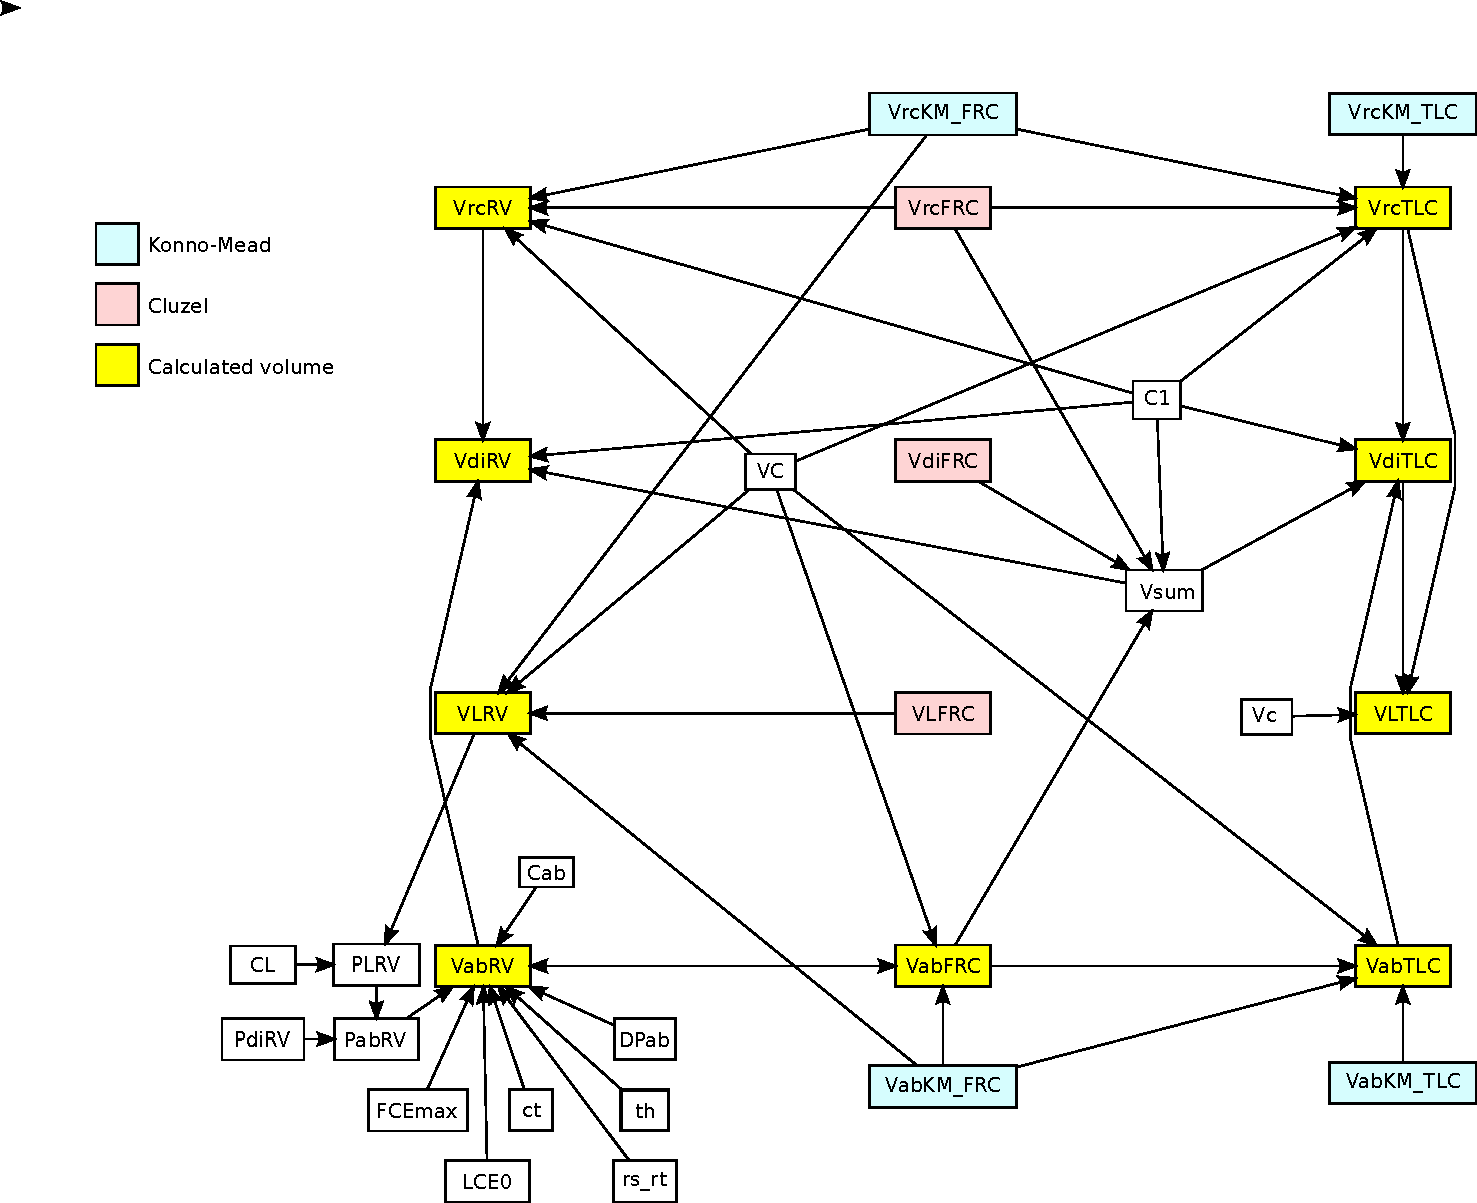
\includegraphics[width=6in]{paramgen.pdf}

\nohyphens{
\bibliographystyle{apalike}
\bibliography{references}
%\printbibliography{references}
}

\end{document}
